%!TEX root = /Users/stevenmartell/Documents/CURRENT PROJECTS/iSCAM-trunk/fba/BC-herring-2011/PRESENTATION/BC-Herring-2011.tex

\section{Part II} % (fold)
\label{sec:part_ii}

\subsection{Introduction} % (fold)
\label{sub:introduction}
%
\begin{frame}[t]\frametitle{Introduction}
	Objectives:
	\begin{enumerate}
		\item Data used in the 2011 assessment.
		\item Overview of the analytical methods.
		\item Present the 2011 stock assessment.
		\item Describe \& present the catch forecasts for 2012.
	\end{enumerate}
\end{frame}

%% subsection introduction (end)

\subsection{2011 Data} % (fold)
\label{sub:2011_data}
%
\begin{frame}[c]\frametitle{Data used in the 2011 stock assessment}
	\begin{itemize}
		\item Catch by gear type.
		\item Spawn survey data.
		\item Age-composition data.
		\item Empirical weight-at-age data. 
	\end{itemize}
\end{frame}
%
\begin{frame}[t]\frametitle{Catch by gear (1950:2011)}
	\only<1>{
	\begin{figure}[htbp]
		\centering
		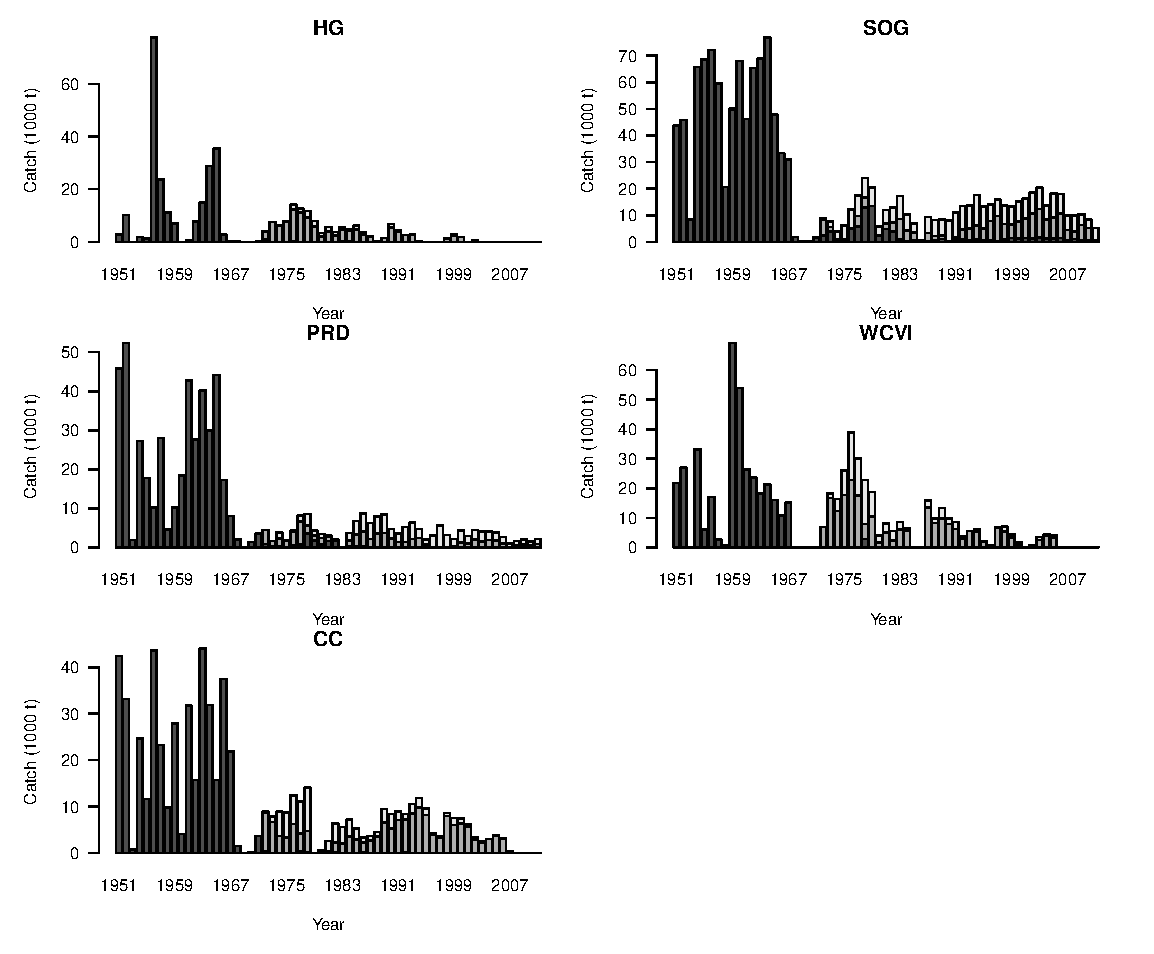
\includegraphics[clip,trim=0 304 300 0 ]
		{../FIGS/iscam_fig_CatchMajorAreas}
		\caption{Catch by gear for Haida Gwaii.}
	\end{figure}
	}
	\only<2>{
	\begin{figure}[htbp]
		\centering
		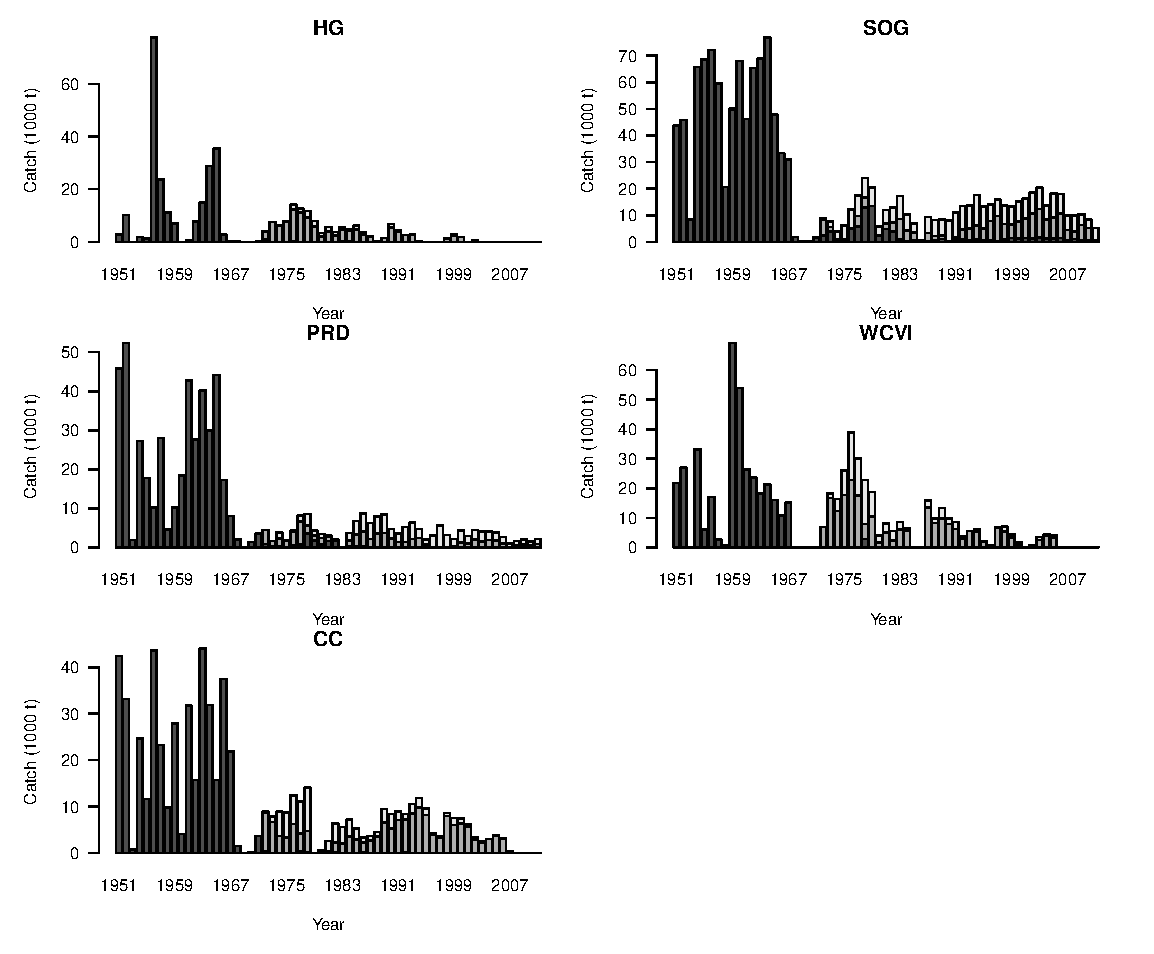
\includegraphics[clip,trim=0 156 300 155 ]
		{../FIGS/iscam_fig_CatchMajorAreas}
		\caption{Catch by gear for Prince Rupert District.}
	\end{figure}
	}
	\only<3>{
	\begin{figure}[htbp]
		\centering
		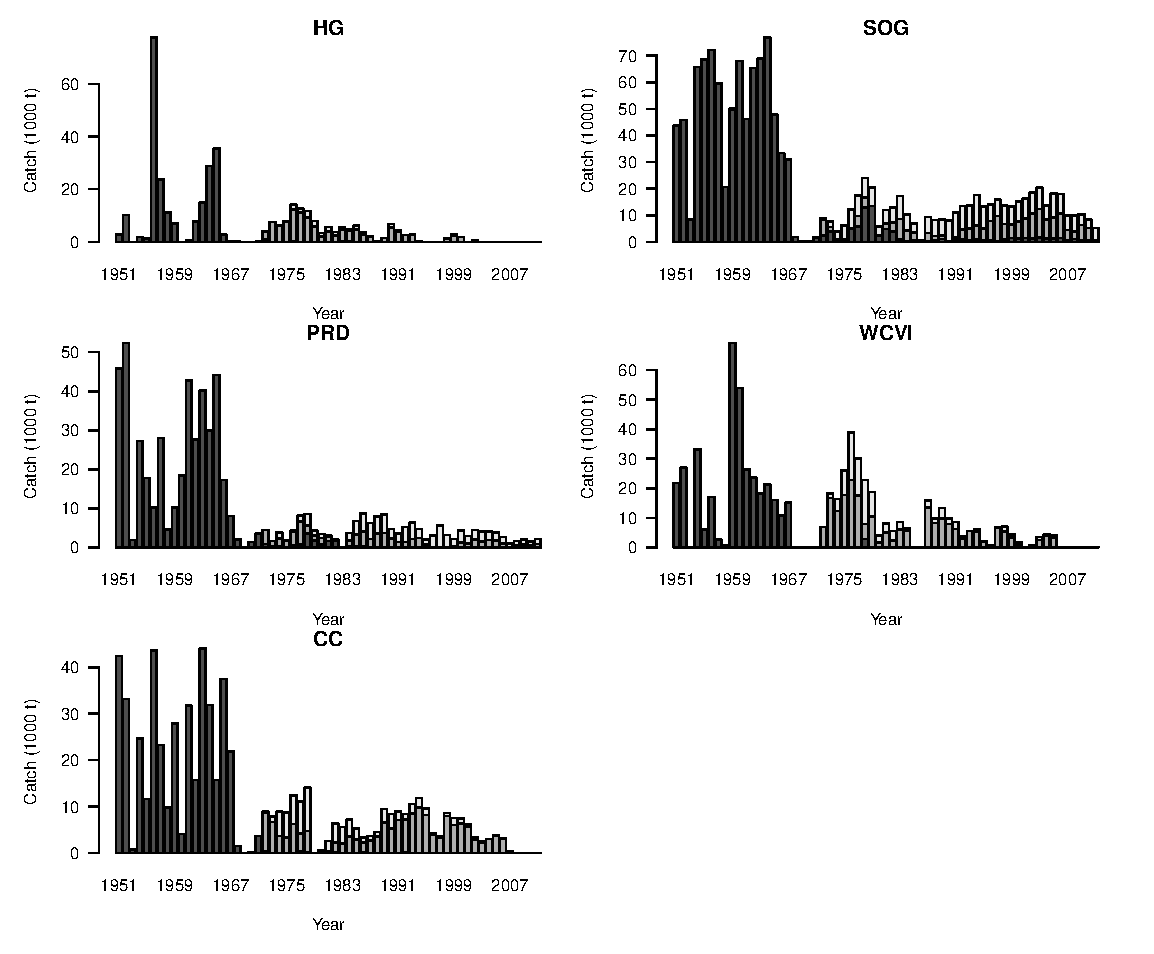
\includegraphics[clip,trim=0 0 300 301 ]
		{../FIGS/iscam_fig_CatchMajorAreas}
		\caption{Catch by gear for Central Coast.}
	\end{figure}
	}
	\only<4>{
	\begin{figure}[htbp]
		\centering
		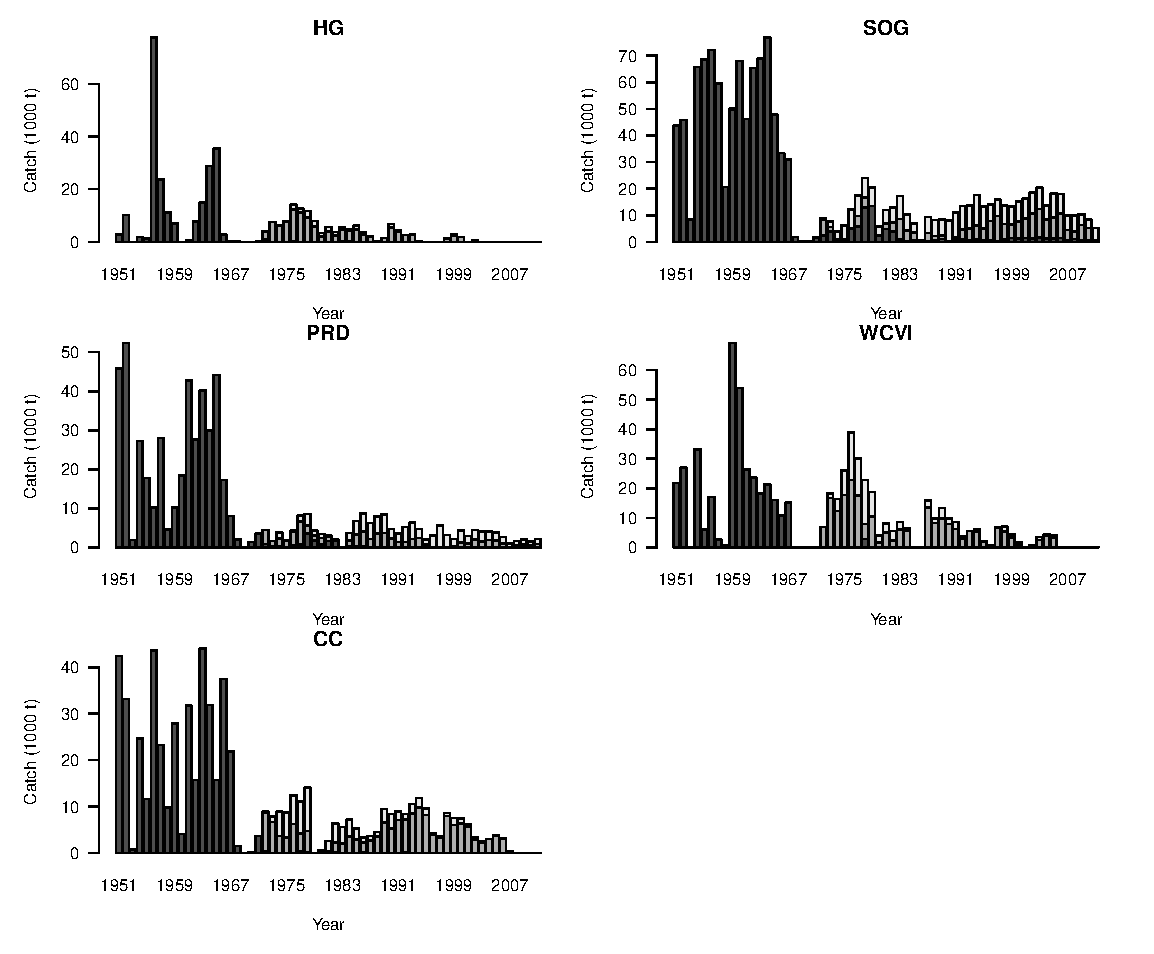
\includegraphics[clip,trim=300 304 0 0 ]
		{../FIGS/iscam_fig_CatchMajorAreas}
		\caption{Catch by gear for Strait of Georgia.}
	\end{figure}
	}
	\only<5>{
	\begin{figure}[htbp]
		\centering
		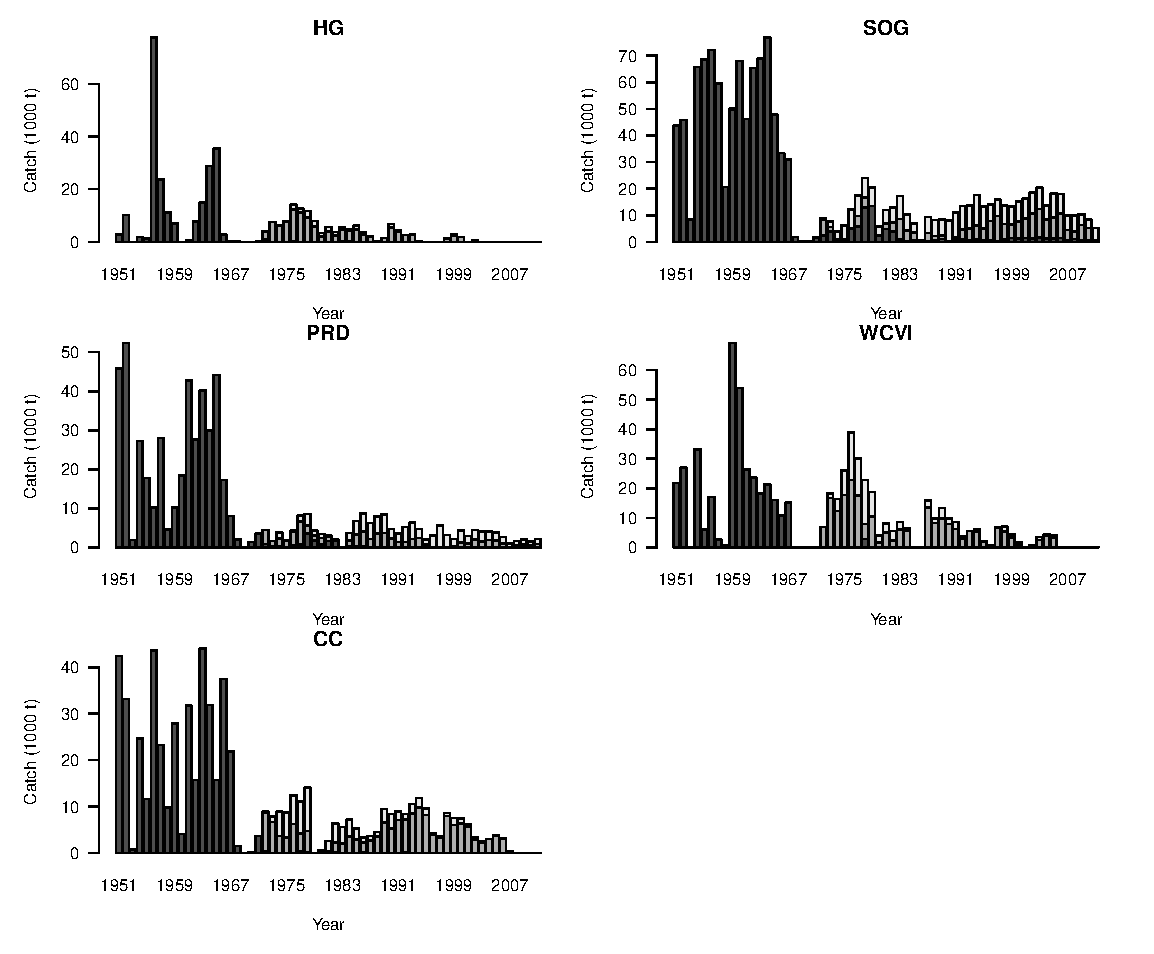
\includegraphics[clip,trim=300 156 0 155 ]
		{../FIGS/iscam_fig_CatchMajorAreas}
		\caption{Catch by gear for West Coast of Vancouver Island.}
	\end{figure}
	}
\end{frame}
%
\begin{frame}[t]\frametitle{Spawning activity in 2010}
	\only<1>{
	\begin{figure}[htbp]
		\centering
		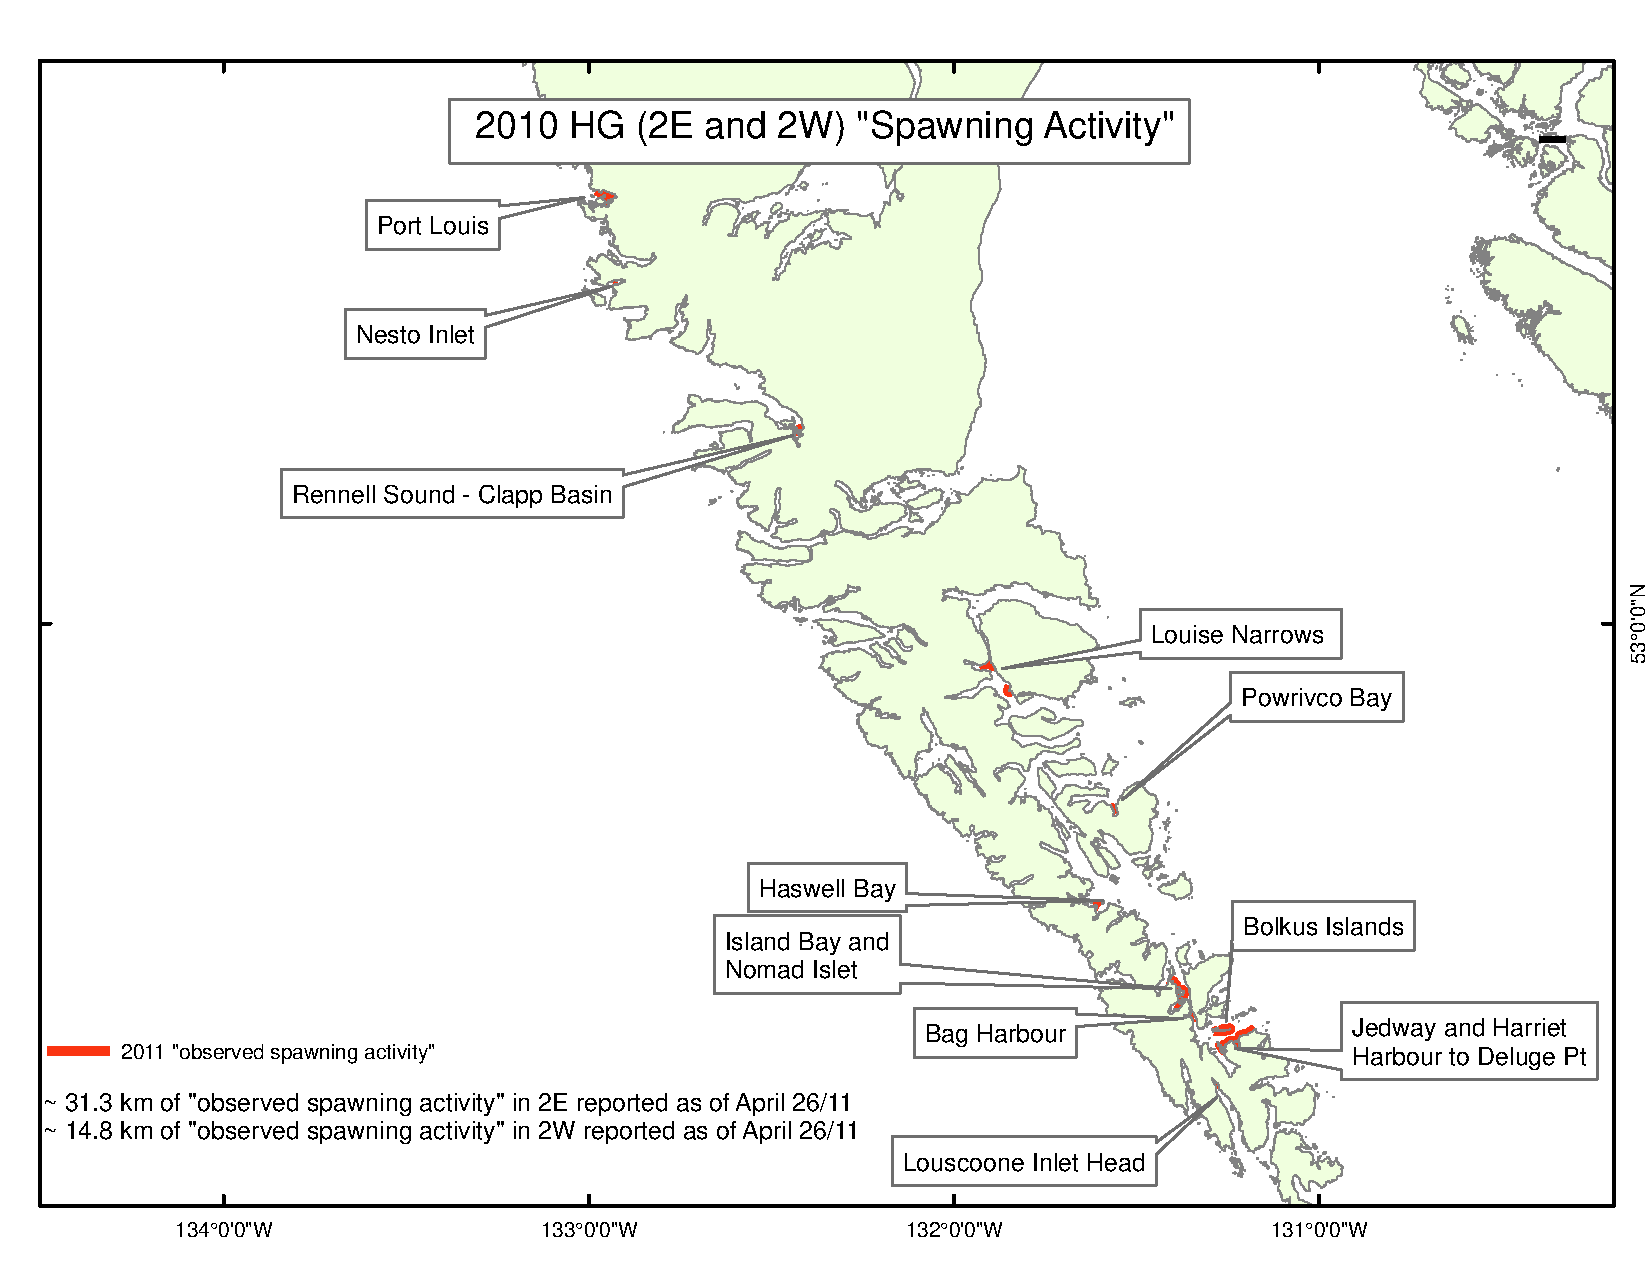
\includegraphics[scale=0.3]
		{../FIGS/PBSfigs/2011-HG-Prelim-WG}
		\caption{2010 Spawning activity in Haida Gwaii.}
	\end{figure}
	}
	\only<2>{
	\begin{figure}[htbp]
		\centering
		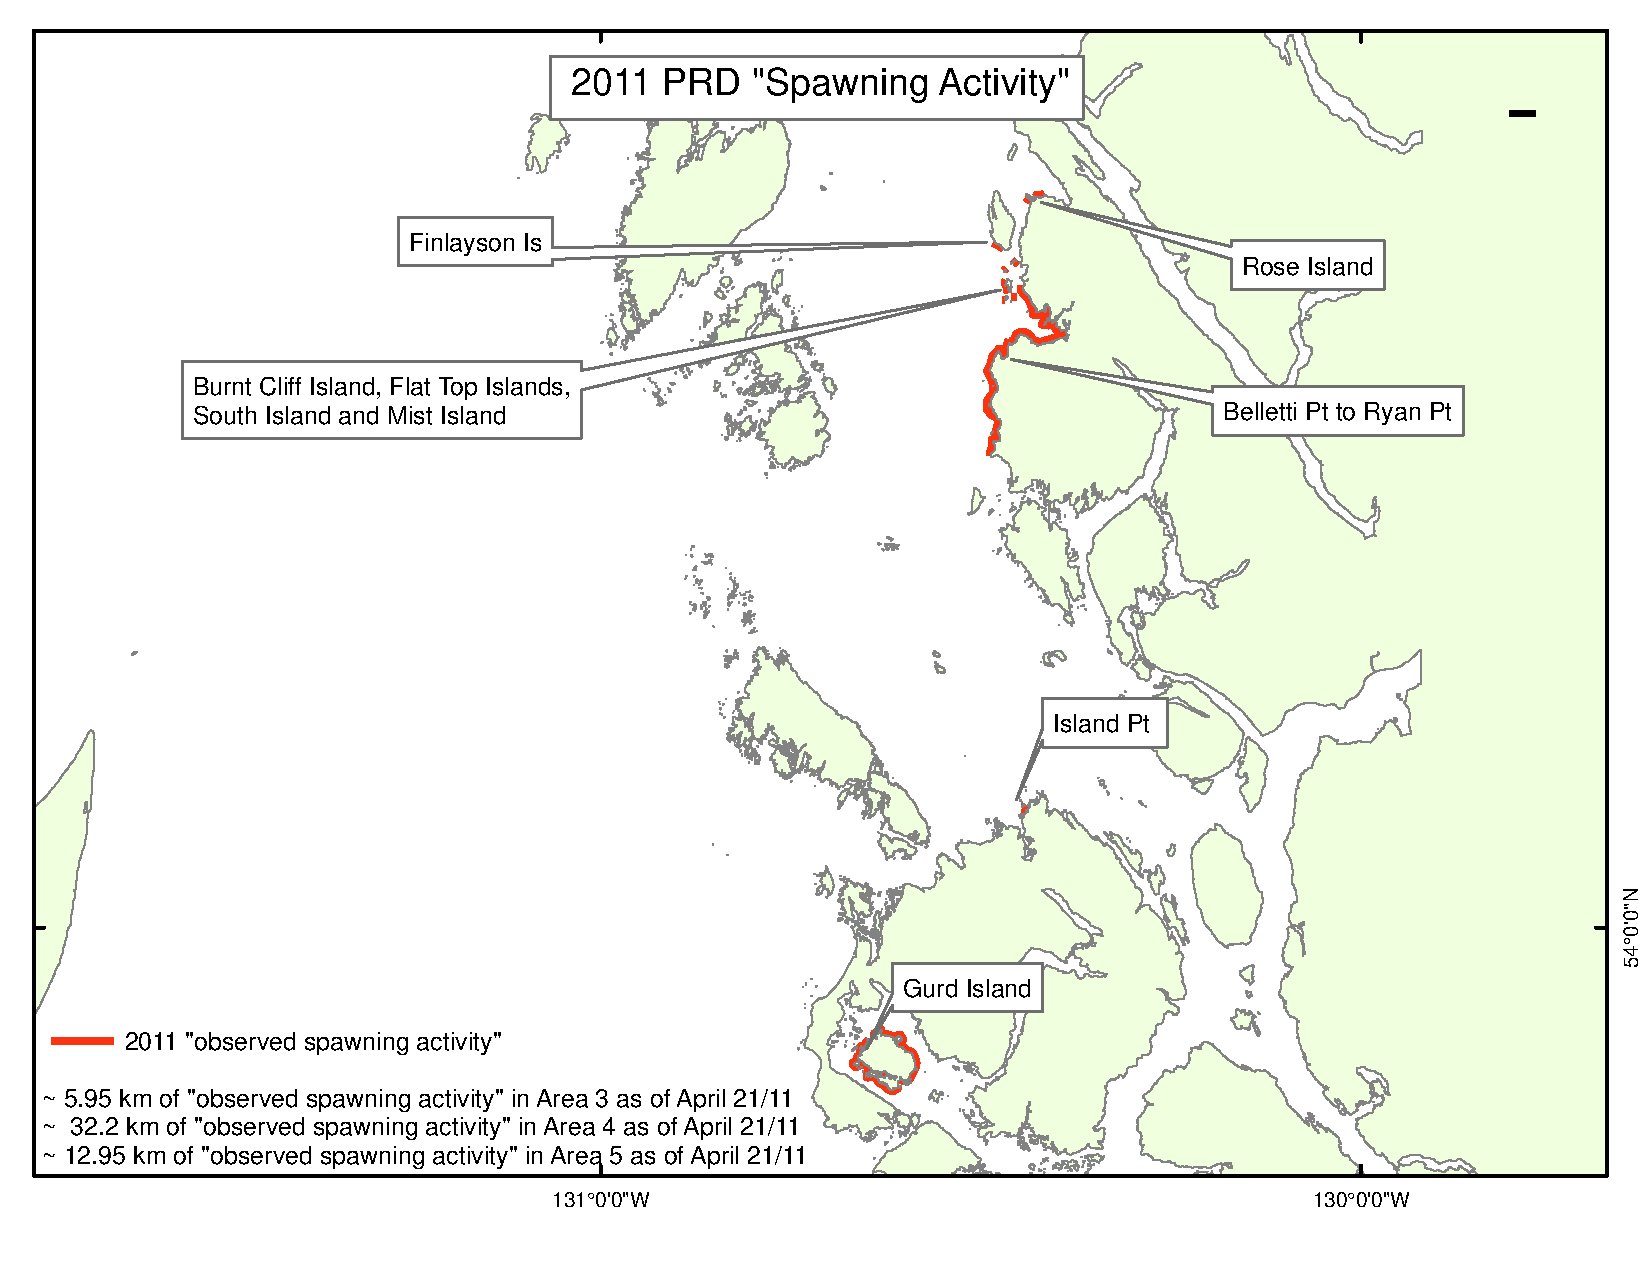
\includegraphics[scale=0.3]
		{../FIGS/PBSfigs/2011-PRD-Prelim-WG}
		\caption{2010 Spawning activity in Prince Rupert District.}
	\end{figure}
	}
	\only<3>{
	\begin{figure}[htbp]
		\centering
		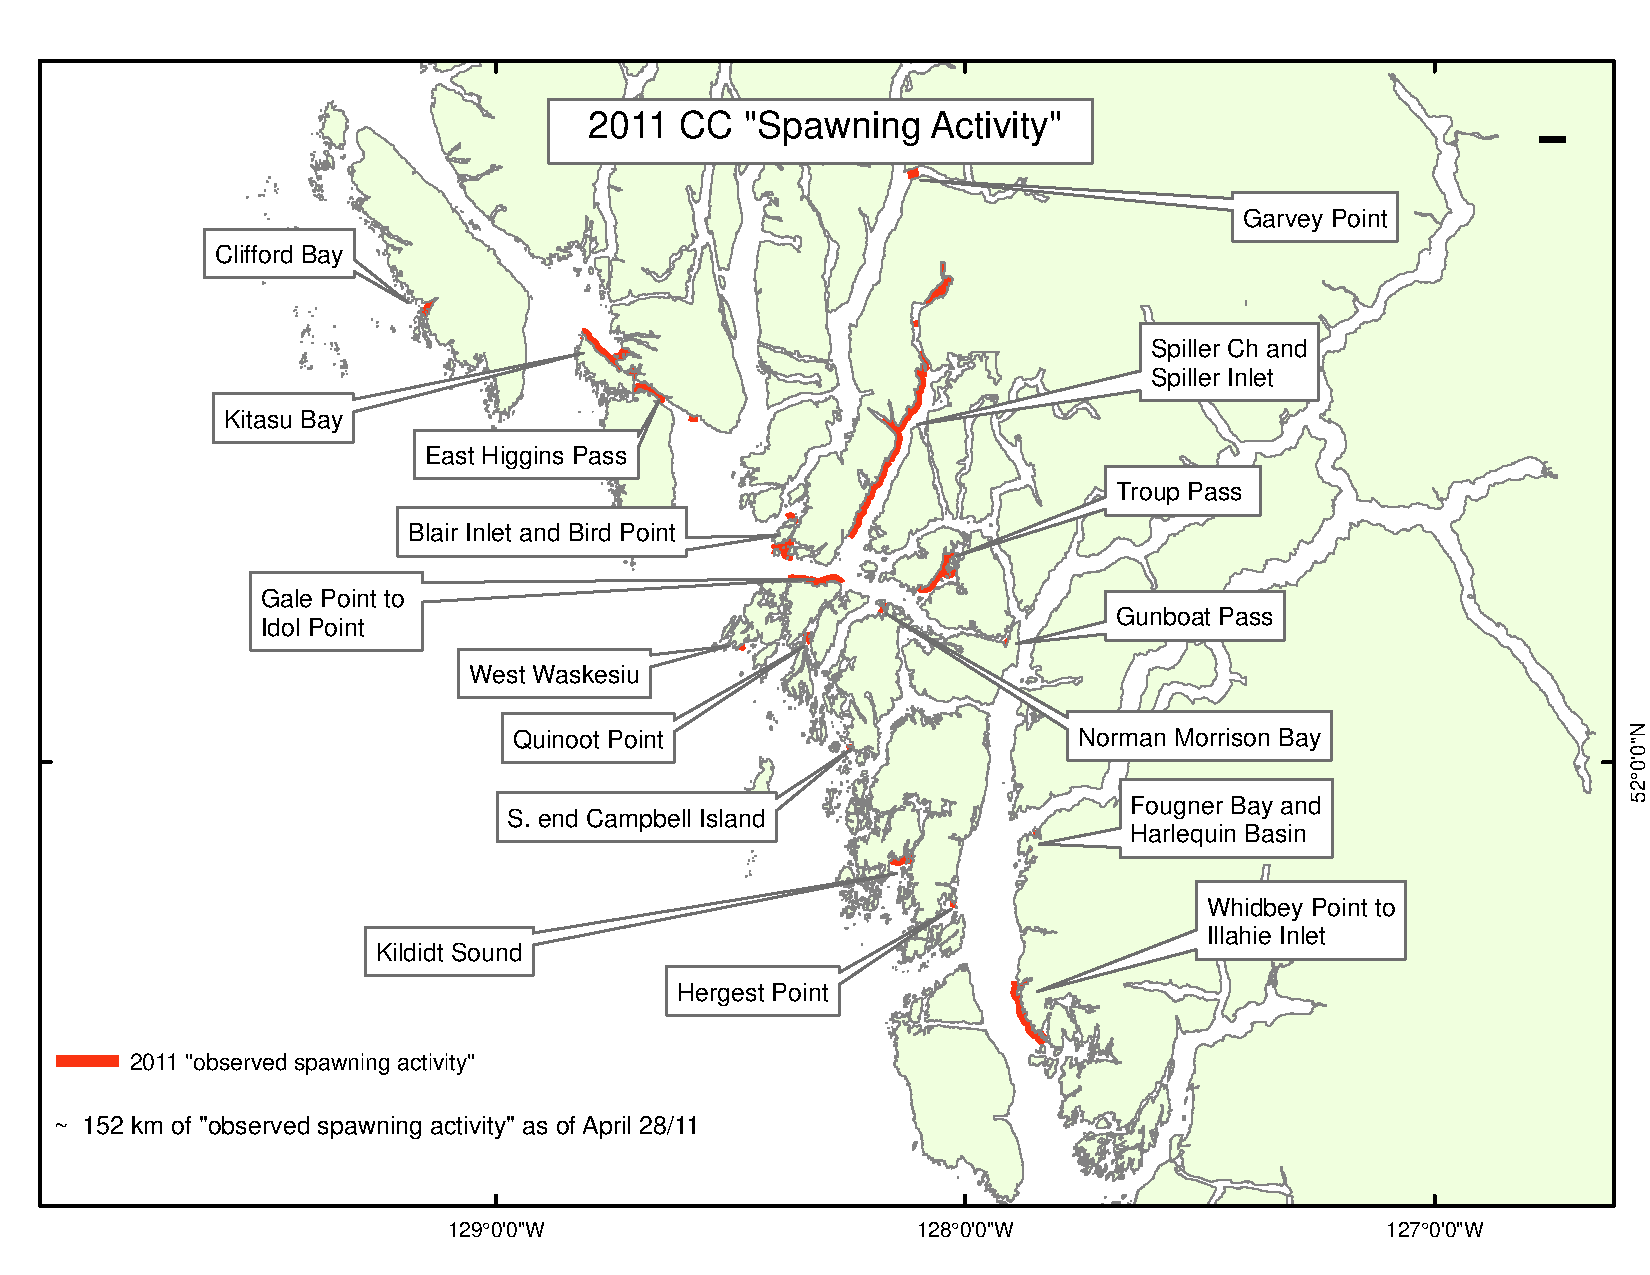
\includegraphics[scale=0.3]
		{../FIGS/PBSfigs/2011-CC-Prelim-WG}
		\caption{2010 Spawning activity in Central Coast.}
	\end{figure}
	}
	\only<4>{
	\begin{figure}[htbp]
		\centering
		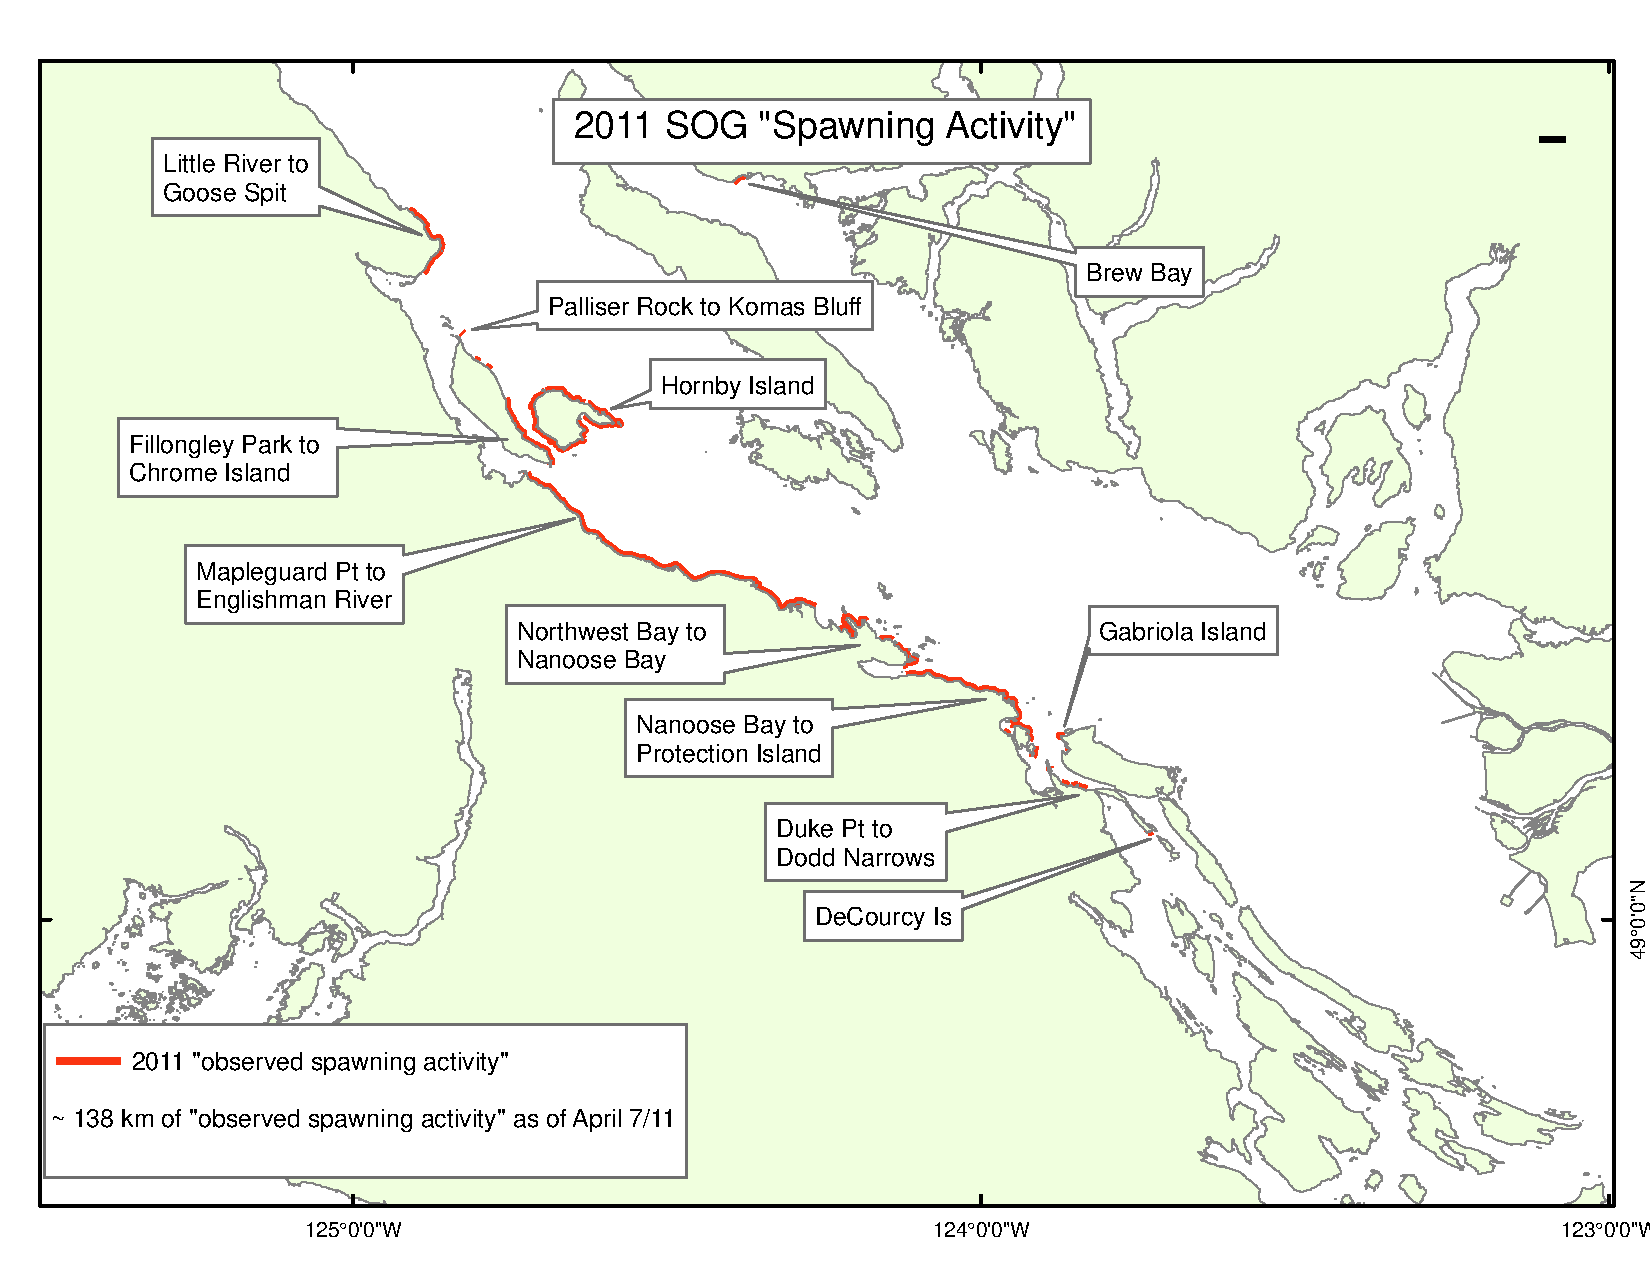
\includegraphics[scale=0.3]
		{../FIGS/PBSfigs/2011-SOG-Prelim-WG}
		\caption{2010 Spawning activity in Strait of Georgia.}
	\end{figure}
	}
	\only<5>{
	\begin{figure}[htbp]
		\centering
		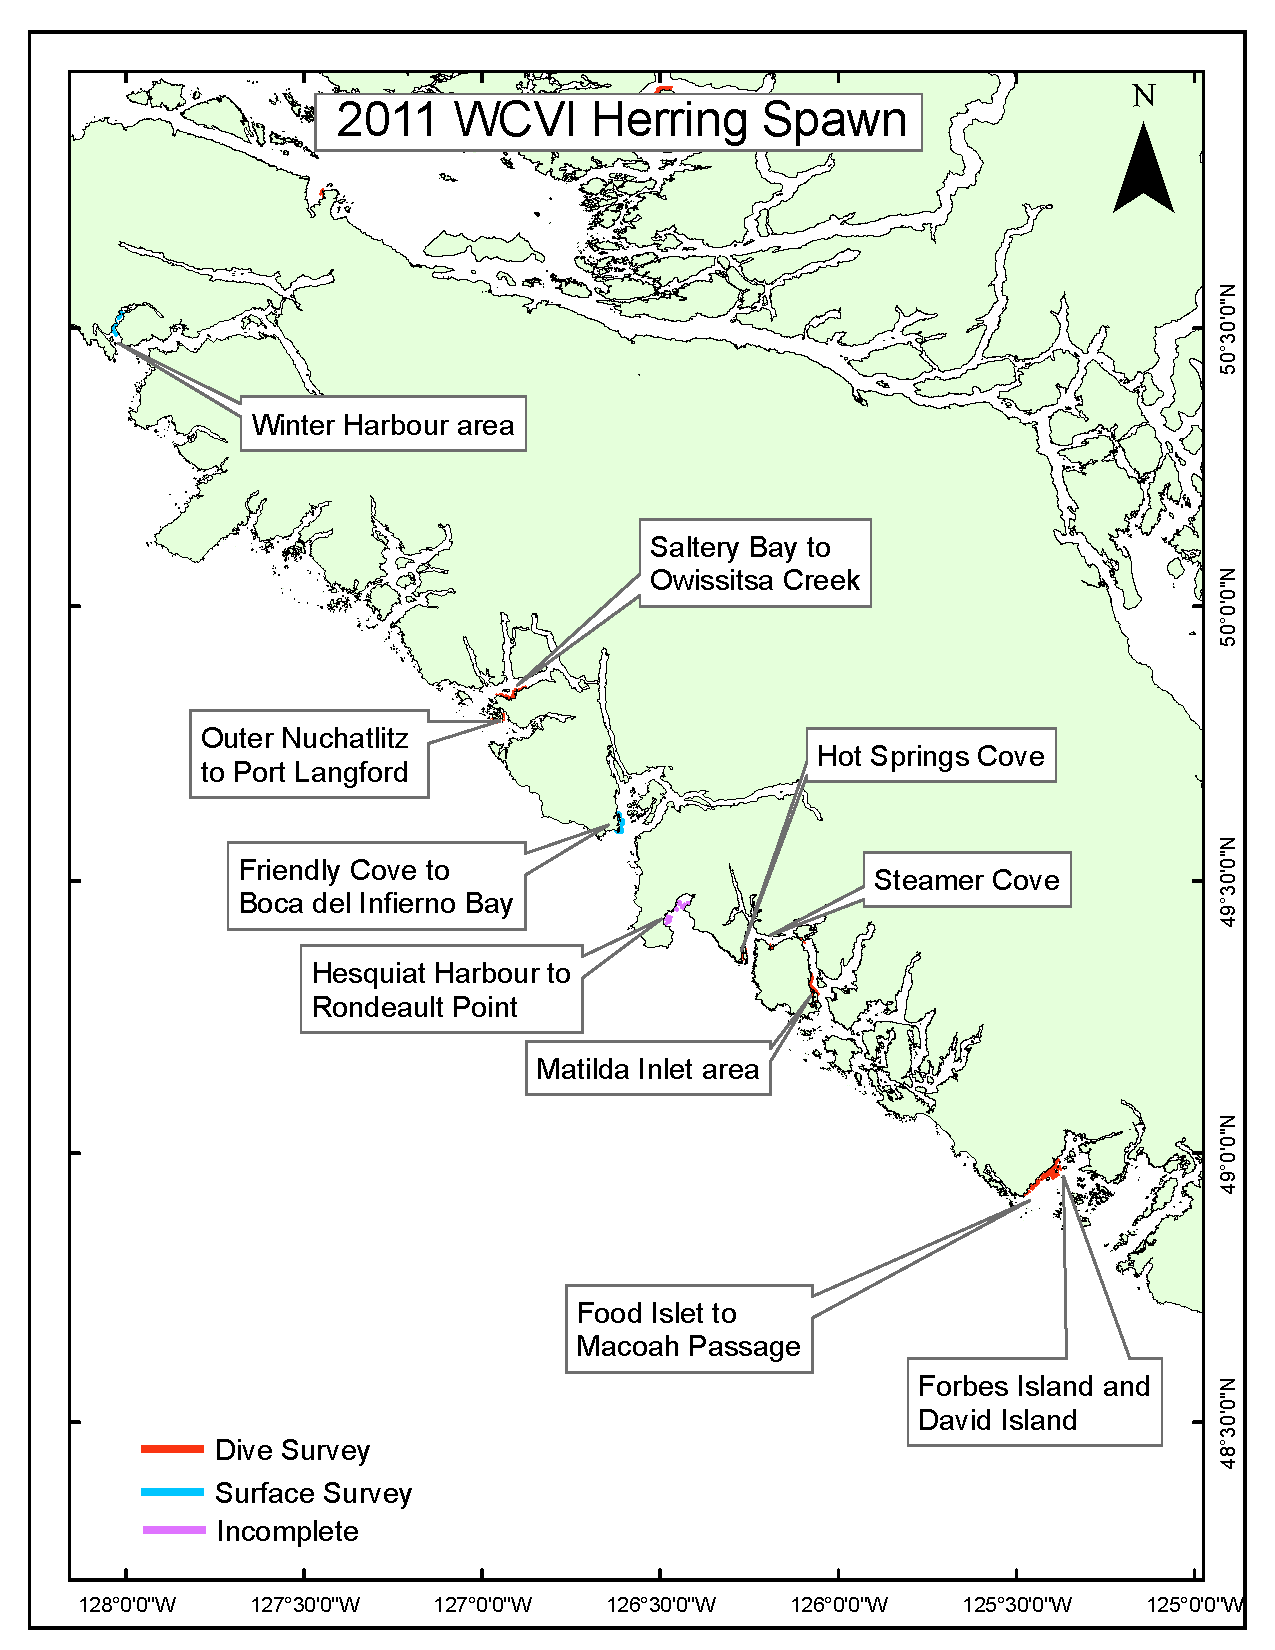
\includegraphics[scale=0.23]
		{../FIGS/PBSfigs/2011_spawn_WCVI_August16}
		\caption{2010 Spawning activity in West Coast Vancouver Island.}
	\end{figure}
	}
\end{frame}
%
\begin{frame}[t]\frametitle{Spawn survey time series}
	\only<1>{
	\begin{figure}[htbp]
		\centering
		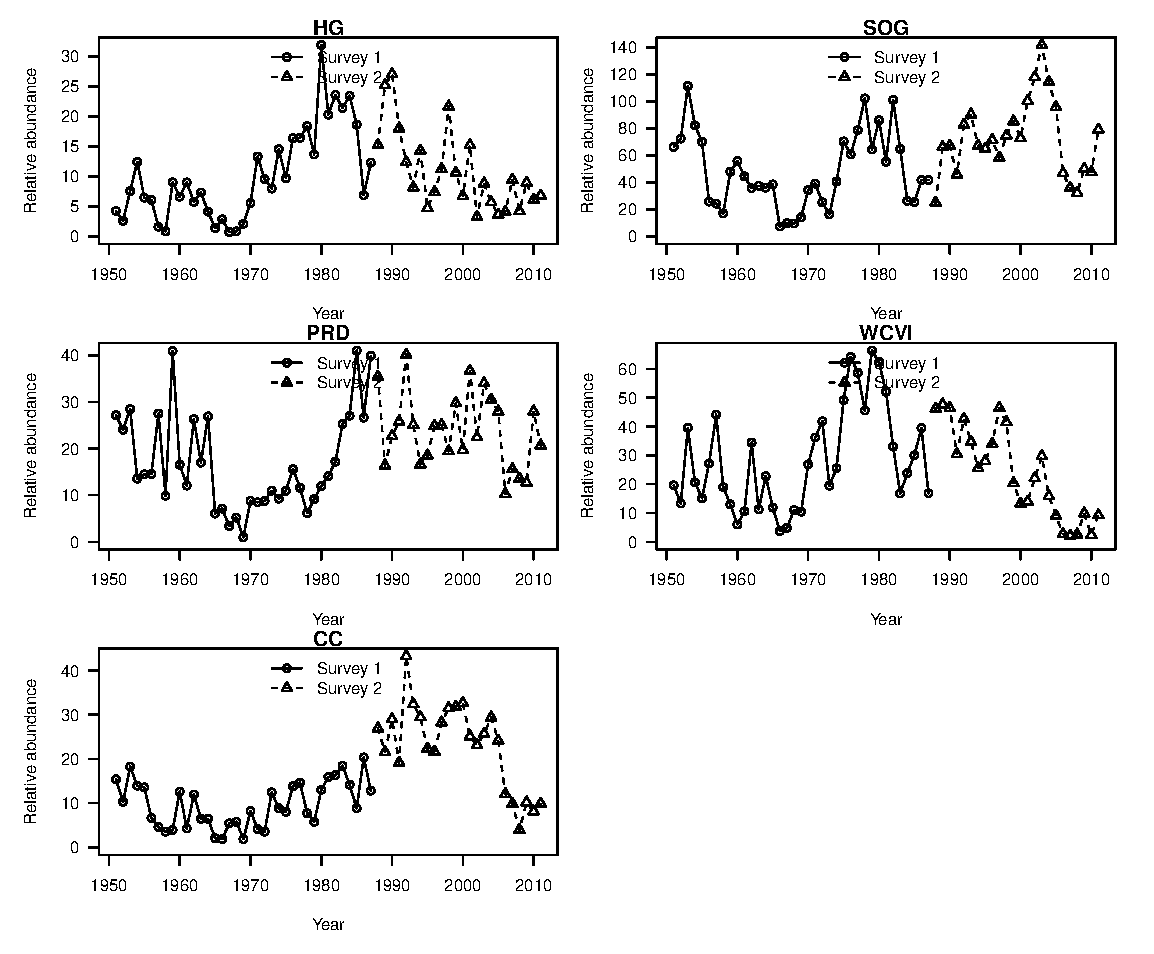
\includegraphics[clip,trim=0 304 275 0]
		{../FIGS/iscam_fig_SurveyMajorAreas}
		\caption{Spawn survey series in Haida Gwaii.}
	\end{figure}
	}
	%
	\only<2>{
	\begin{figure}[htbp]
		\centering
		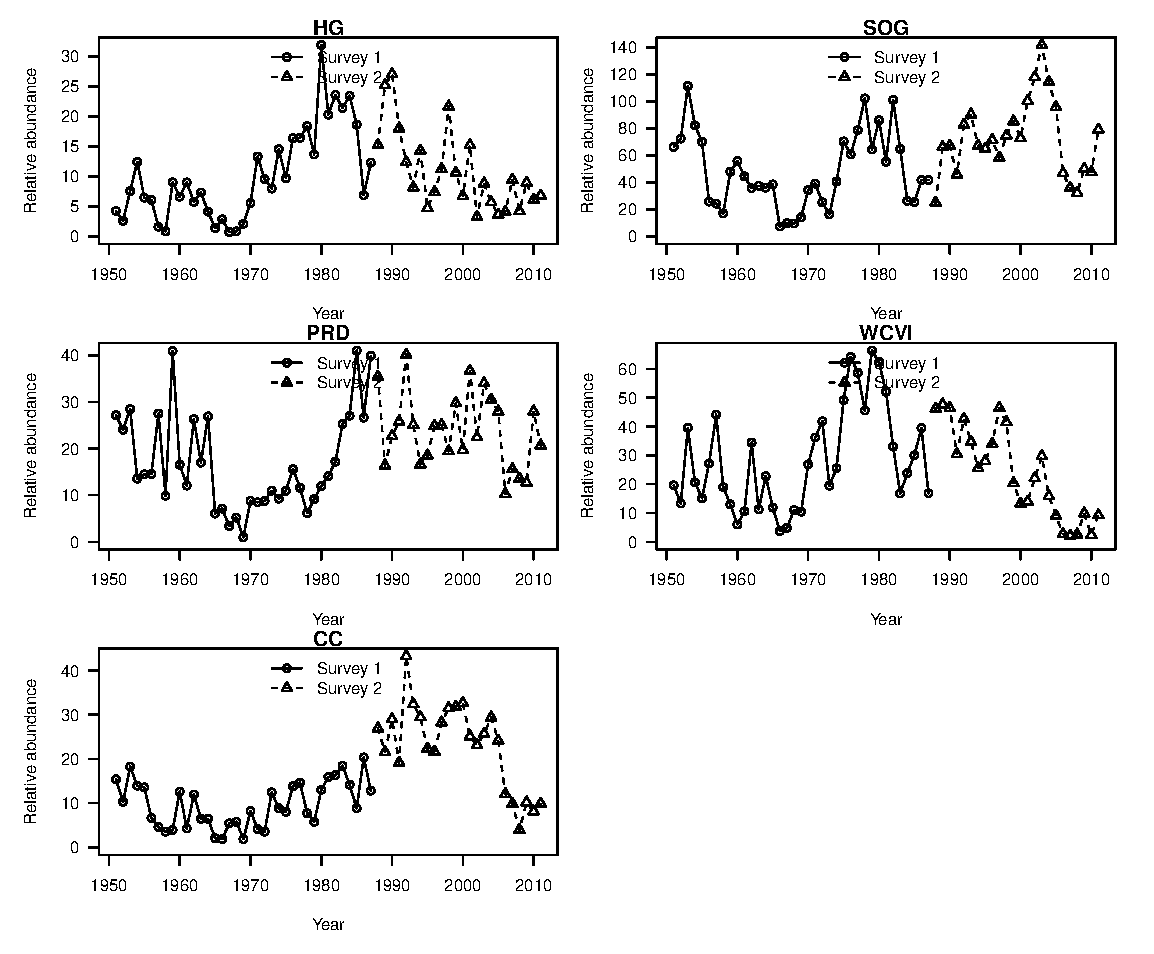
\includegraphics[clip,trim=0 156 275 155]
		{../FIGS/iscam_fig_SurveyMajorAreas}
		\caption{Spawn survey series in Prince Rupert District.}
	\end{figure}
	}
	%
	\only<3>{
	\begin{figure}[htbp]
		\centering
		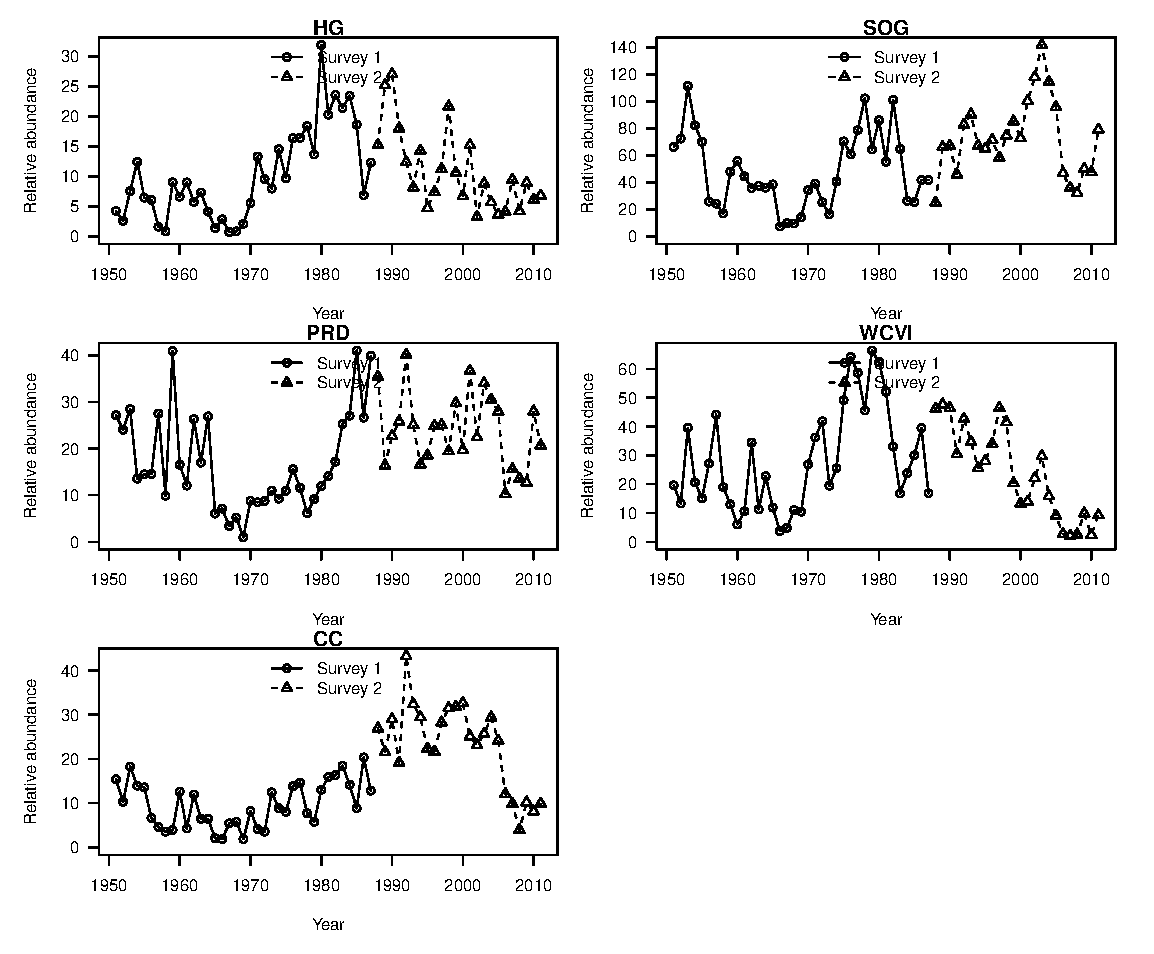
\includegraphics[clip,trim=0 0 275 301]
		{../FIGS/iscam_fig_SurveyMajorAreas}
		\caption{Spawn survey series in Central Coast.}
	\end{figure}
	}
	%
	\only<4>{
	\begin{figure}[htbp]
		\centering
		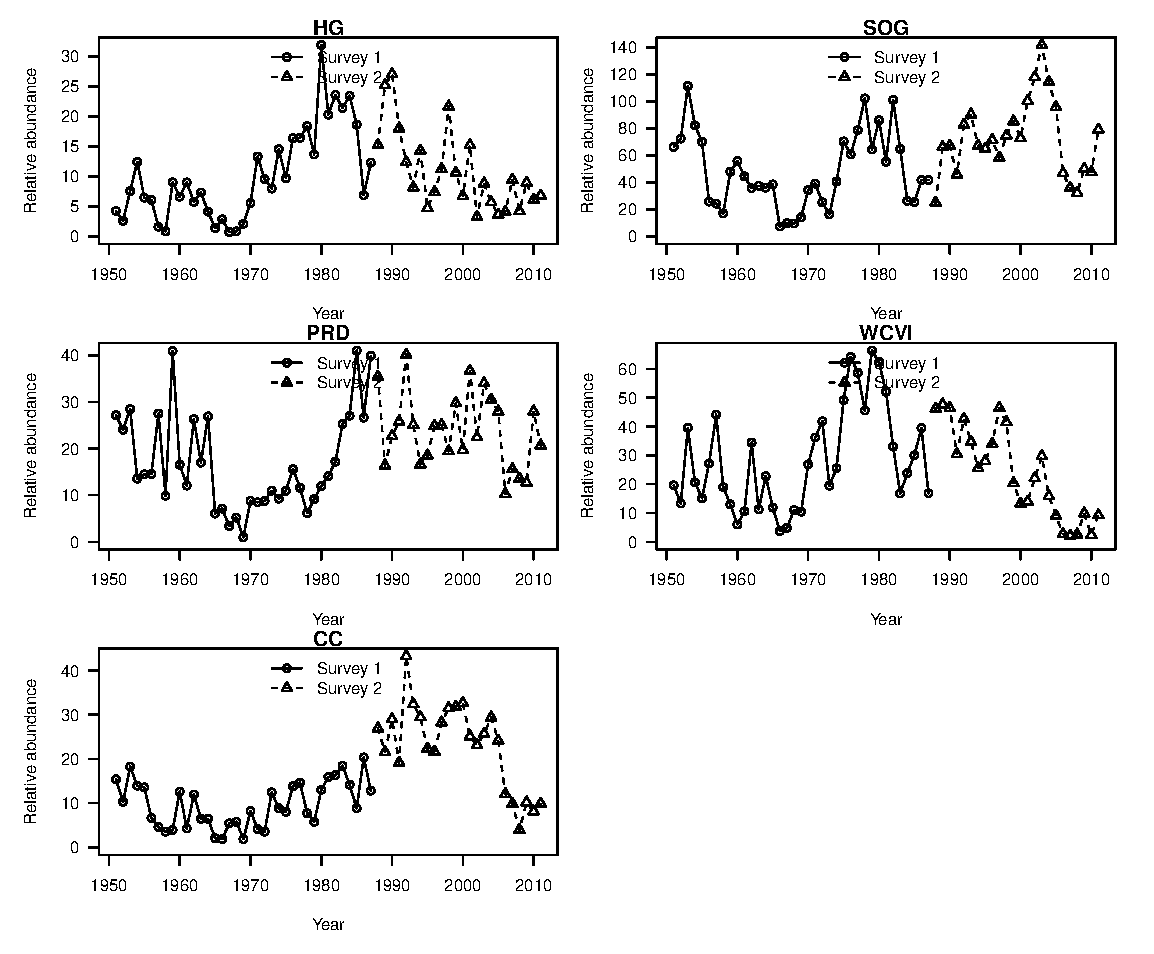
\includegraphics[clip,trim=275 304 0 0]
		{../FIGS/iscam_fig_SurveyMajorAreas}
		\caption{Spawn survey series in Strait of Georgia.}
	\end{figure}
	}
	%
	\only<5>{
	\begin{figure}[htbp]
		\centering
		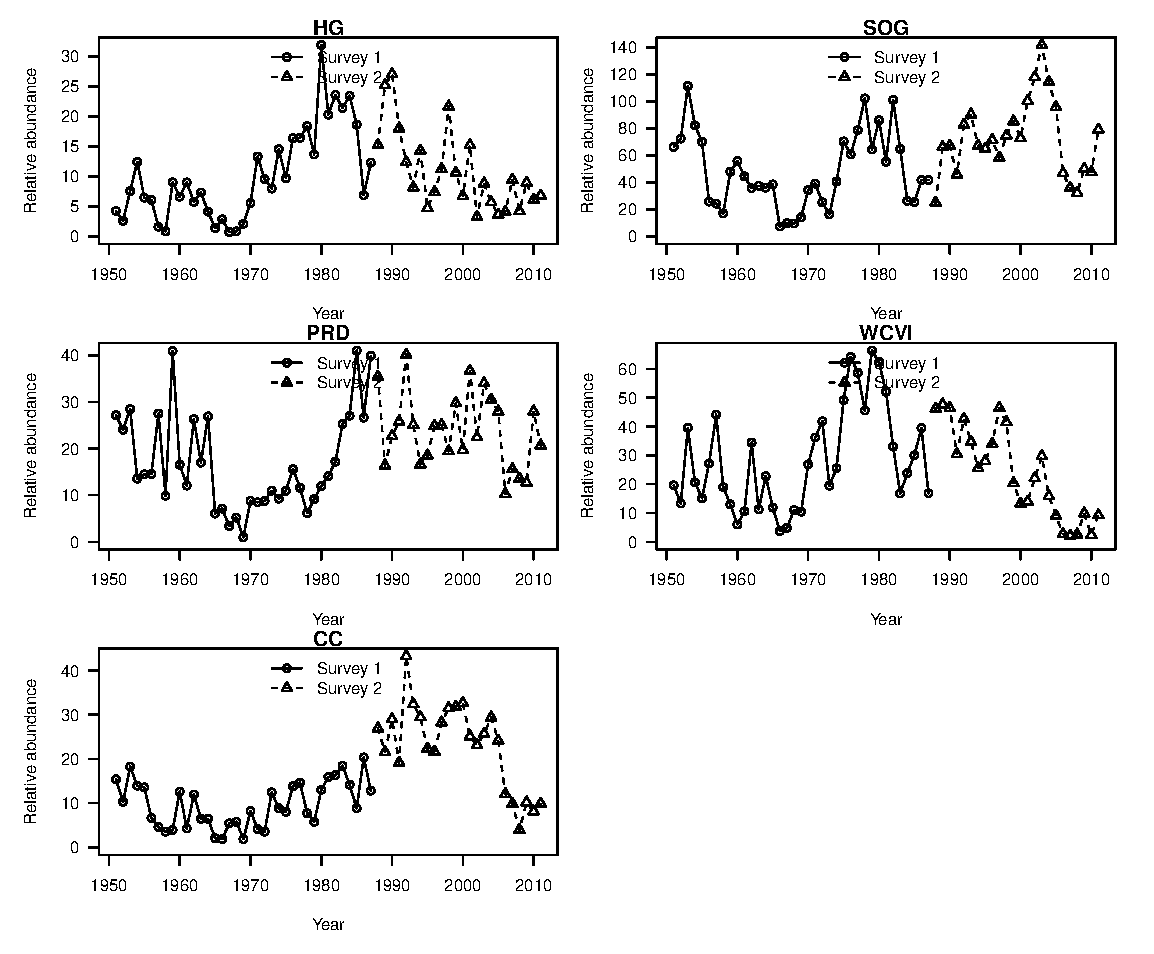
\includegraphics[clip,trim=275 156 0 155]
		{../FIGS/iscam_fig_SurveyMajorAreas}
		\caption{Spawn survey series in West Coast of Vancouver Island.}
	\end{figure}
	}
\end{frame}
%
\begin{frame}[t]\frametitle{Age-composition data}
	\only<1>{
	\begin{figure}[htbp]
		\centering
		\vspace{-0.5cm}	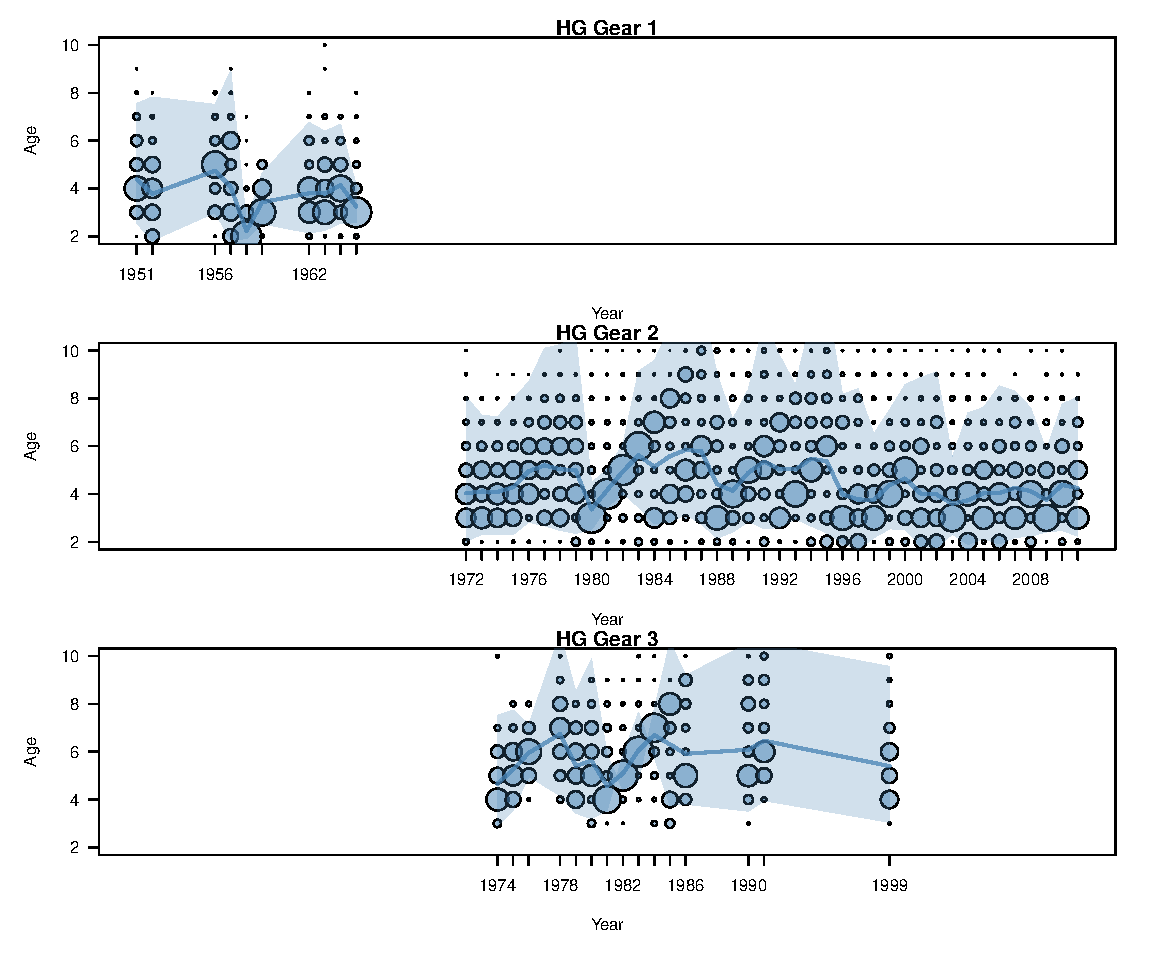
\includegraphics
		[height=0.85\textheight,width=\textwidth]
		{../FIGS/iscam_fig_AgeCompsHG}
		\vspace{-1cm}
		\caption{Haida Gwaii: winter seine, seine-roe, gillnet.}
	\end{figure}
	}
	%
	\only<2>{
	\begin{figure}[htbp]
		\centering
		\vspace{-0.5cm}	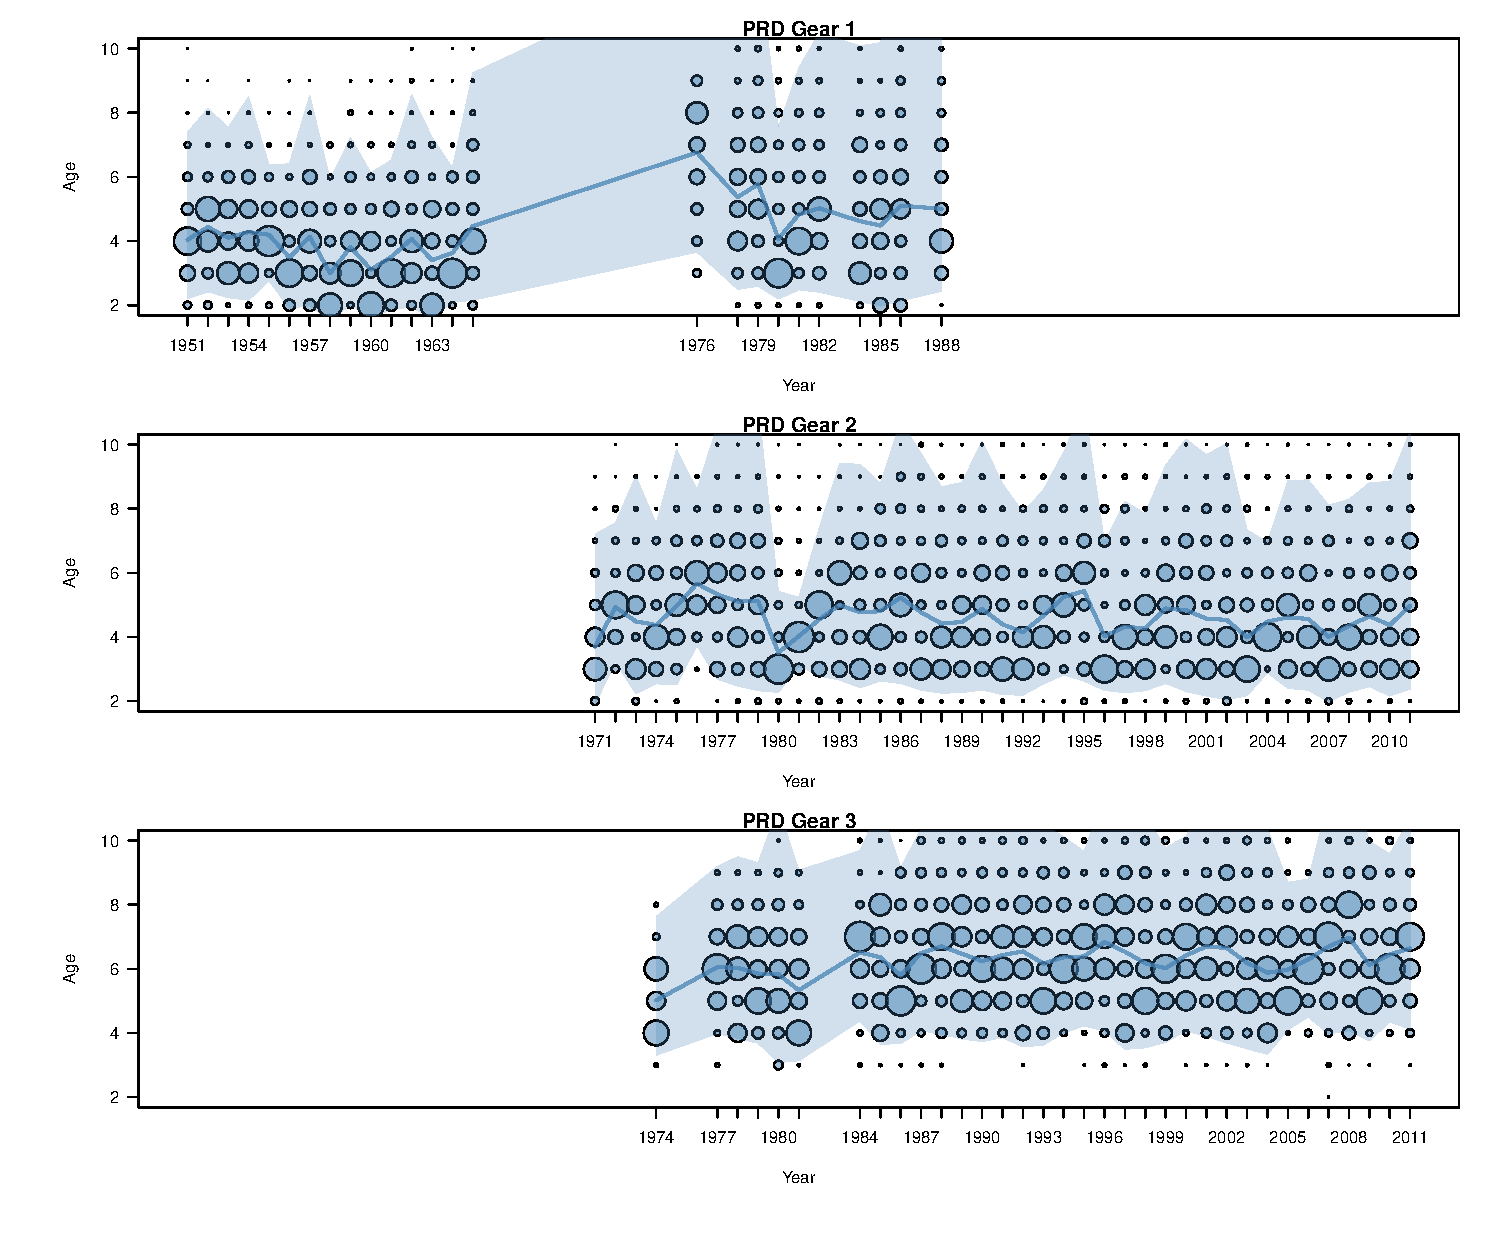
\includegraphics
		[height=0.85\textheight,width=\textwidth]
		{../FIGS/iscam_fig_AgeCompsPRD}
		\vspace{-1cm}
		\caption{Prince Rupert District: winter seine, seine-roe, gillnet.}
	\end{figure}
	}
	%
	\only<3>{
	\begin{figure}[htbp]
		\centering
		\vspace{-0.5cm}	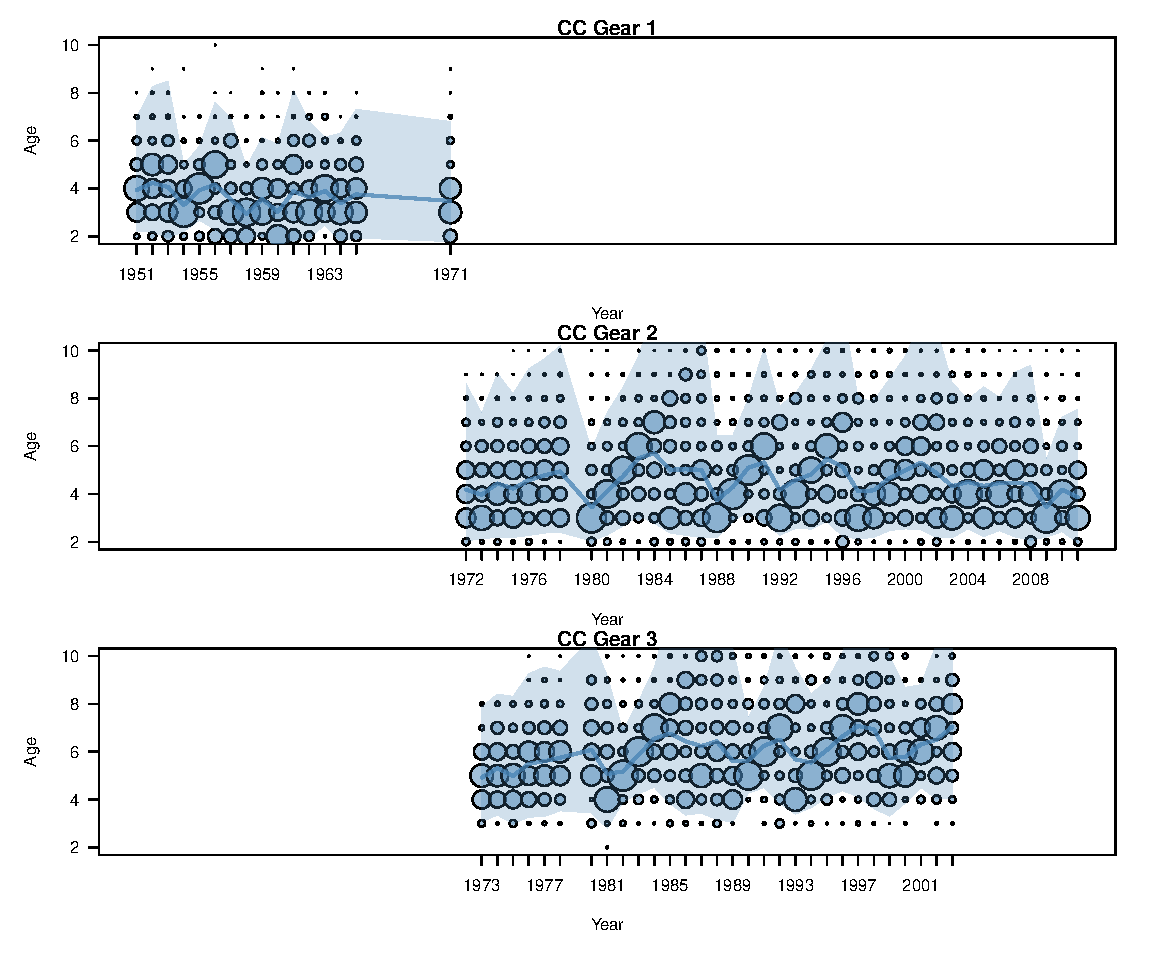
\includegraphics
		[height=0.85\textheight,width=\textwidth]
		{../FIGS/iscam_fig_AgeCompsCC}
		\vspace{-1cm}
		\caption{Central Coast: winter seine, seine-roe, gillnet.}
	\end{figure}
	}
	%
	\only<4>{
	\begin{figure}[htbp]
		\centering
		\vspace{-0.5cm}	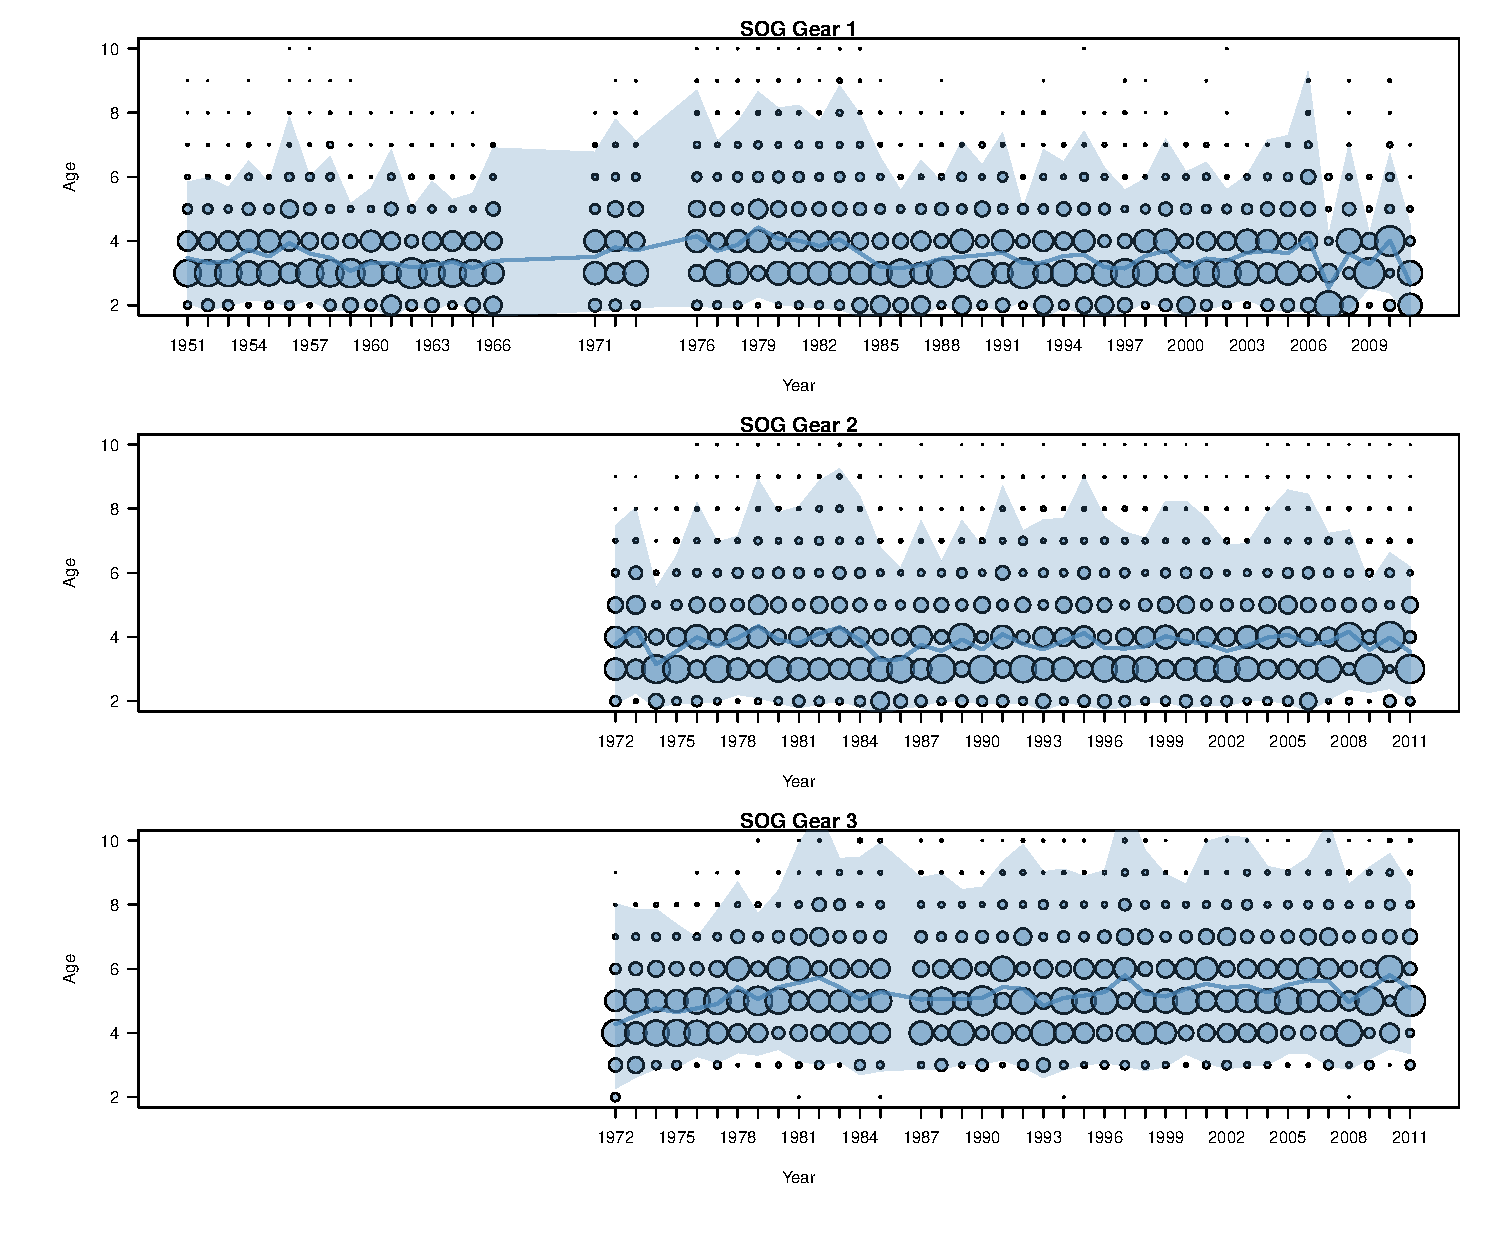
\includegraphics
		[height=0.85\textheight,width=\textwidth]
		{../FIGS/iscam_fig_AgeCompsSOG}
		\vspace{-1cm}
		\caption{Strait of Georgia: winter seine, seine-roe, gillnet.}
	\end{figure}
	}
	%
	\only<5>{
	\begin{figure}[htbp]
		\centering
		\vspace{-0.5cm}	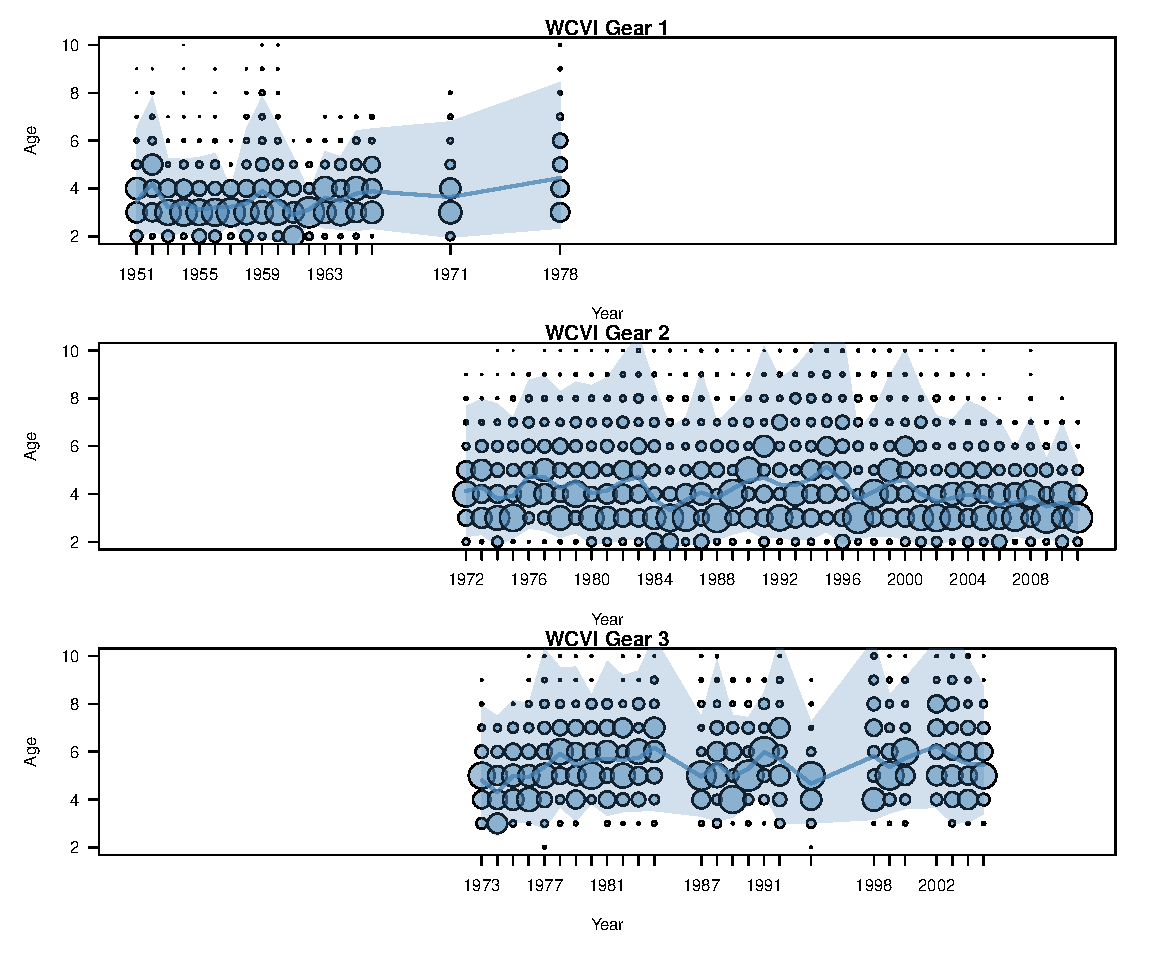
\includegraphics
		[height=0.85\textheight,width=\textwidth]
		{../FIGS/iscam_fig_AgeCompsWCVI}
		\vspace{-1cm}
		\caption{West Coast Vancouver Island: winter seine, seine-roe, gillnet.}
	\end{figure}
	}
	
\end{frame}
%
\begin{frame}[t]\frametitle{Weight-at-age}
	\only<1>{
	\begin{figure}[htbp]
		\centering
		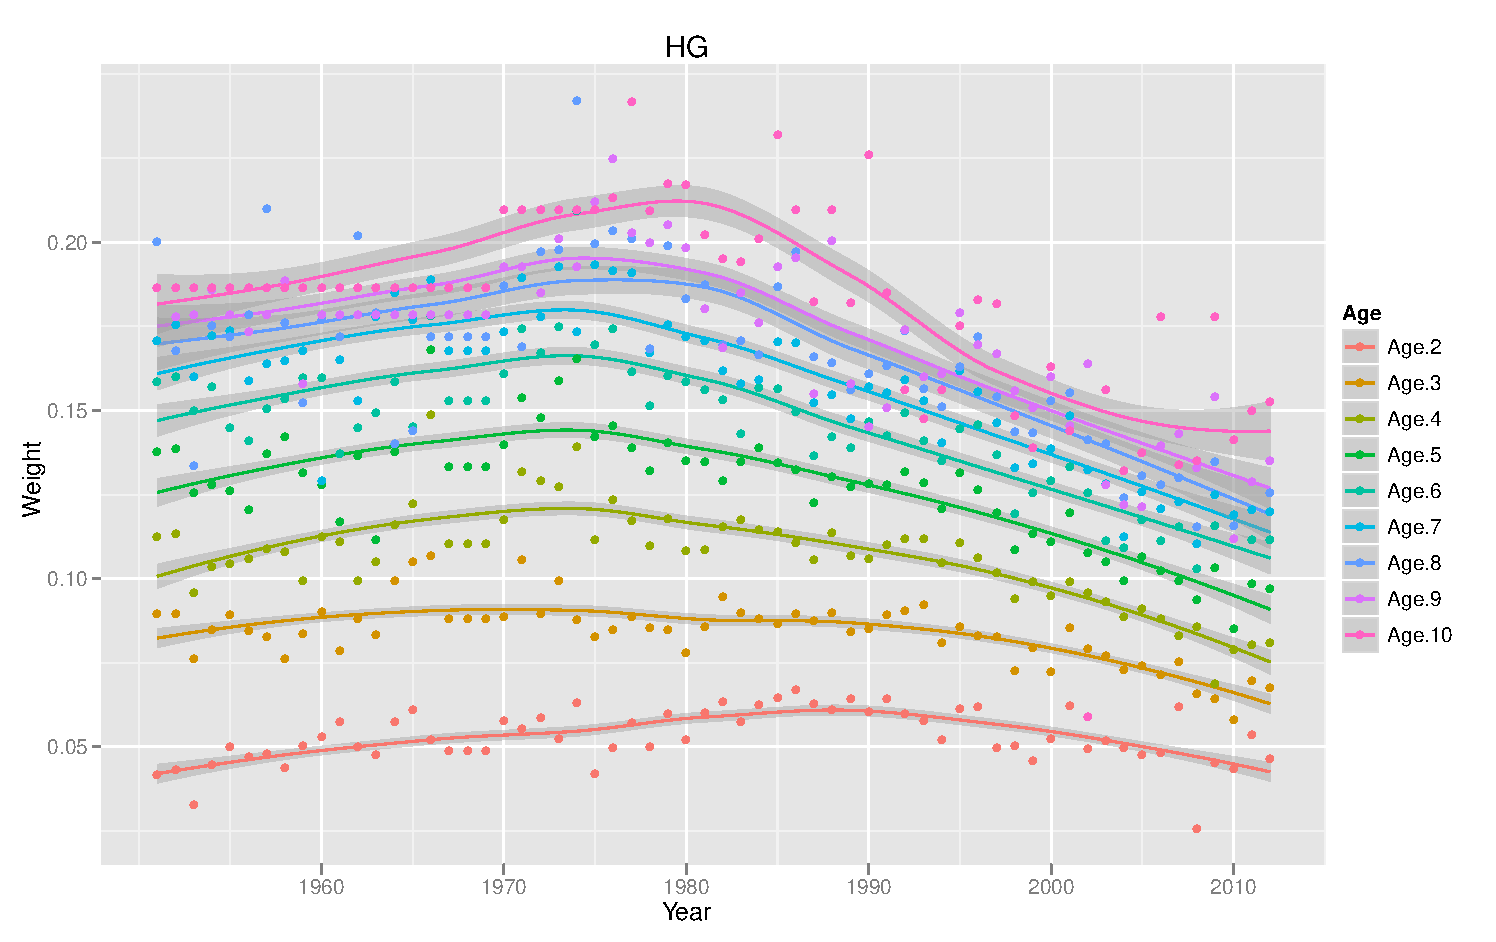
\includegraphics[scale=0.4]
		{../FIGS/iscam_fig_weight-at-age_HG}
		\caption{Haida Gwaii: empirical weight-at-age (kg).}
	\end{figure}
	}
	%
	\only<2>{
	\begin{figure}[htbp]
		\centering
		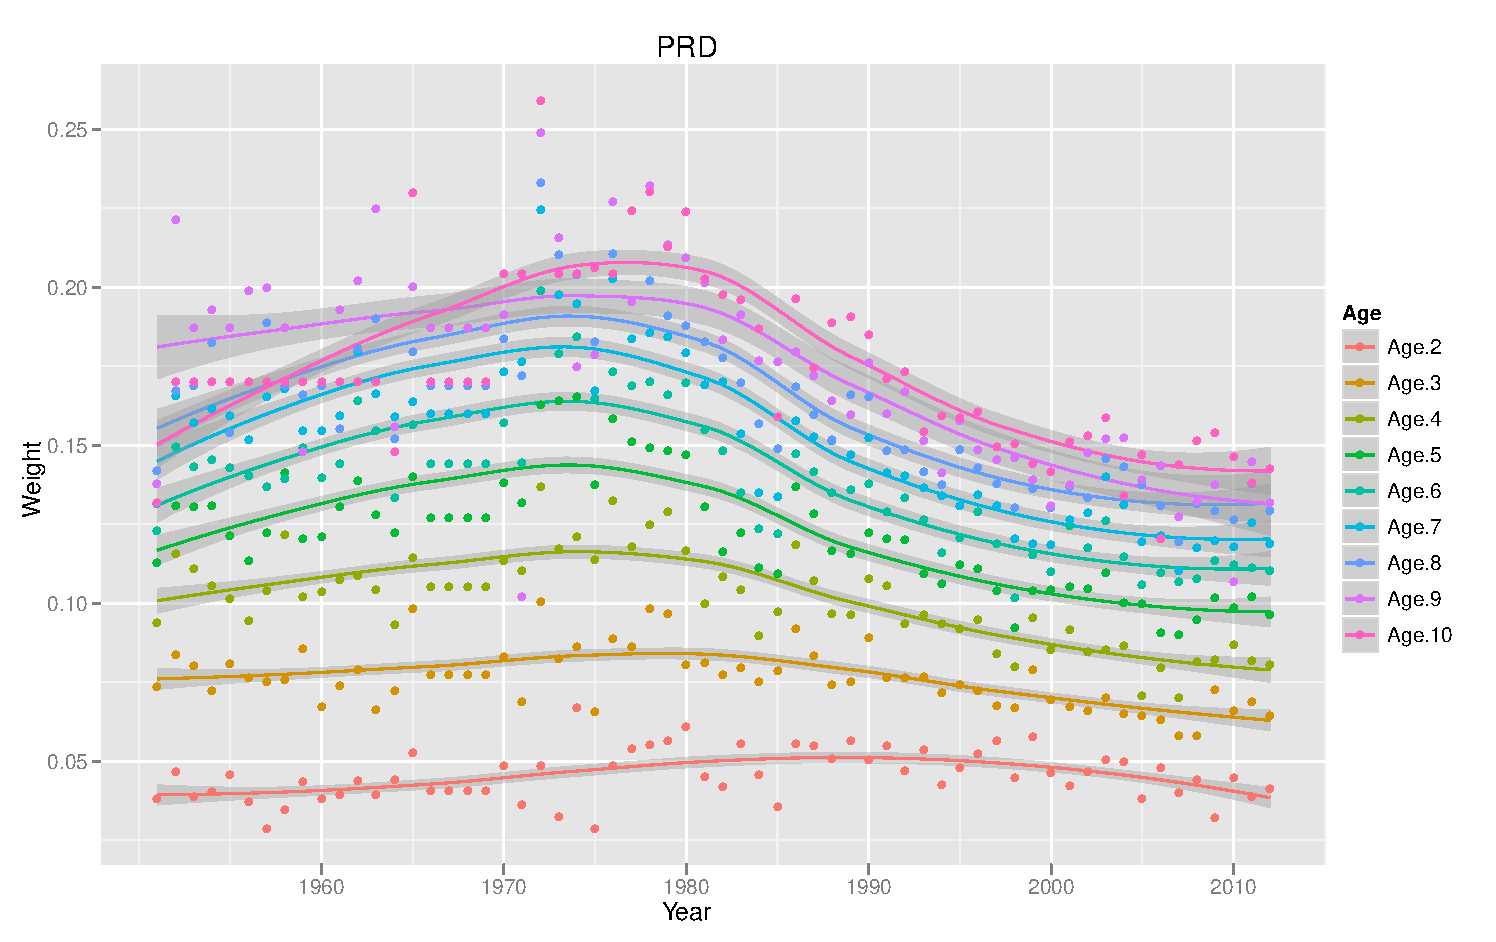
\includegraphics[scale=0.4]
		{../FIGS/iscam_fig_weight-at-age_PRD}
		\caption{Prince Rupert District: empirical weight-at-age (kg).}
	\end{figure}
	}
	%
	\only<3>{
	\begin{figure}[htbp]
		\centering
		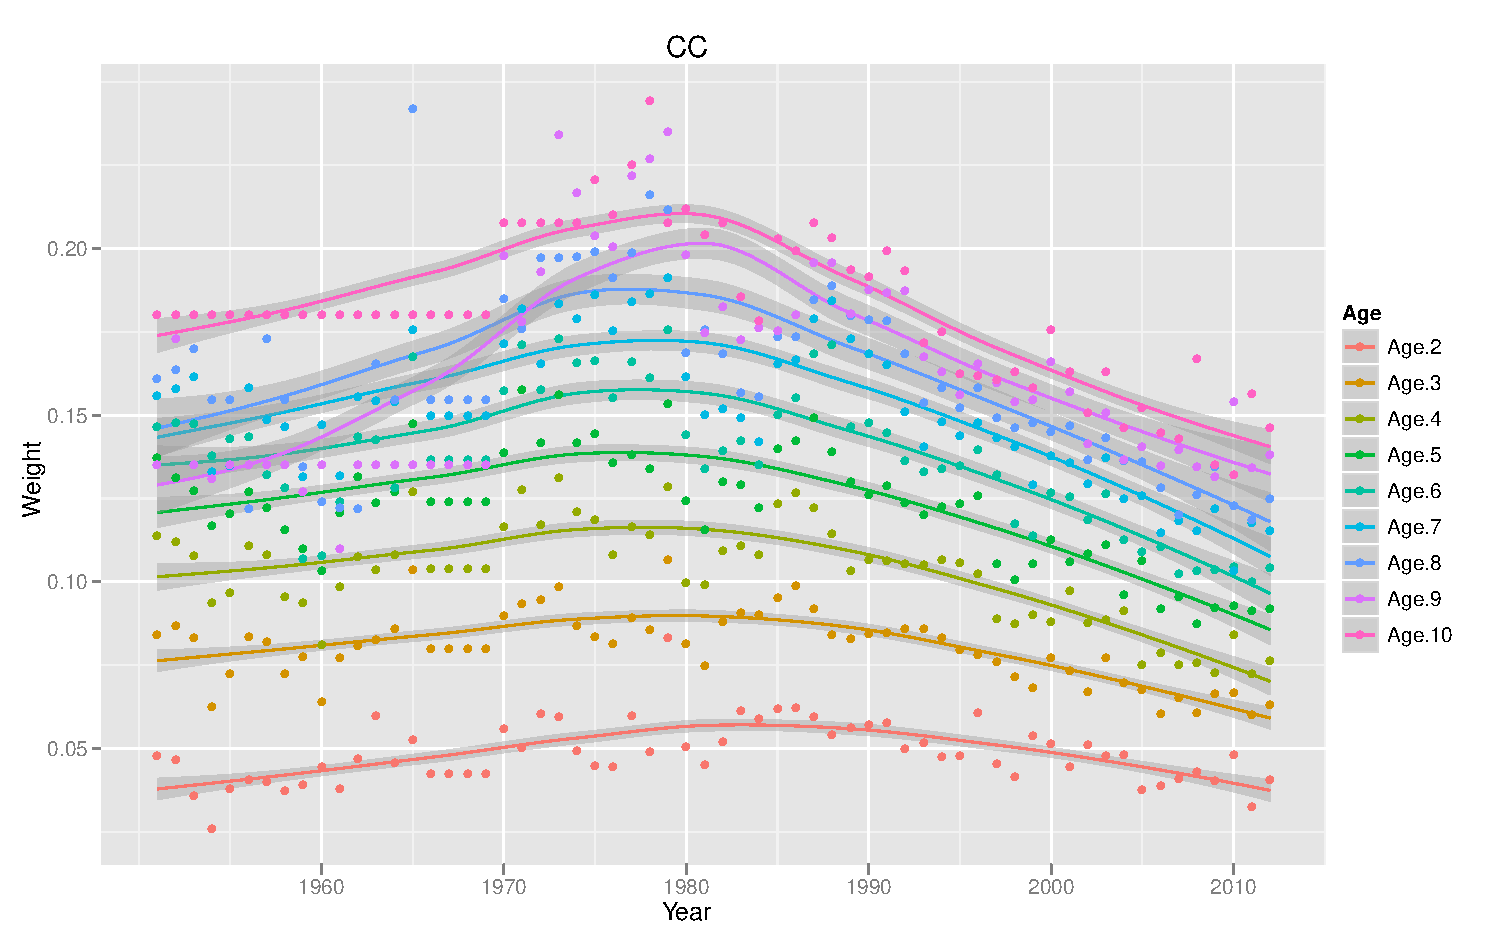
\includegraphics[scale=0.4]
		{../FIGS/iscam_fig_weight-at-age_CC}
		\caption{Central Coast: empirical weight-at-age (kg).}
	\end{figure}
	}
	%
	\only<4>{
	\begin{figure}[htbp]
		\centering
		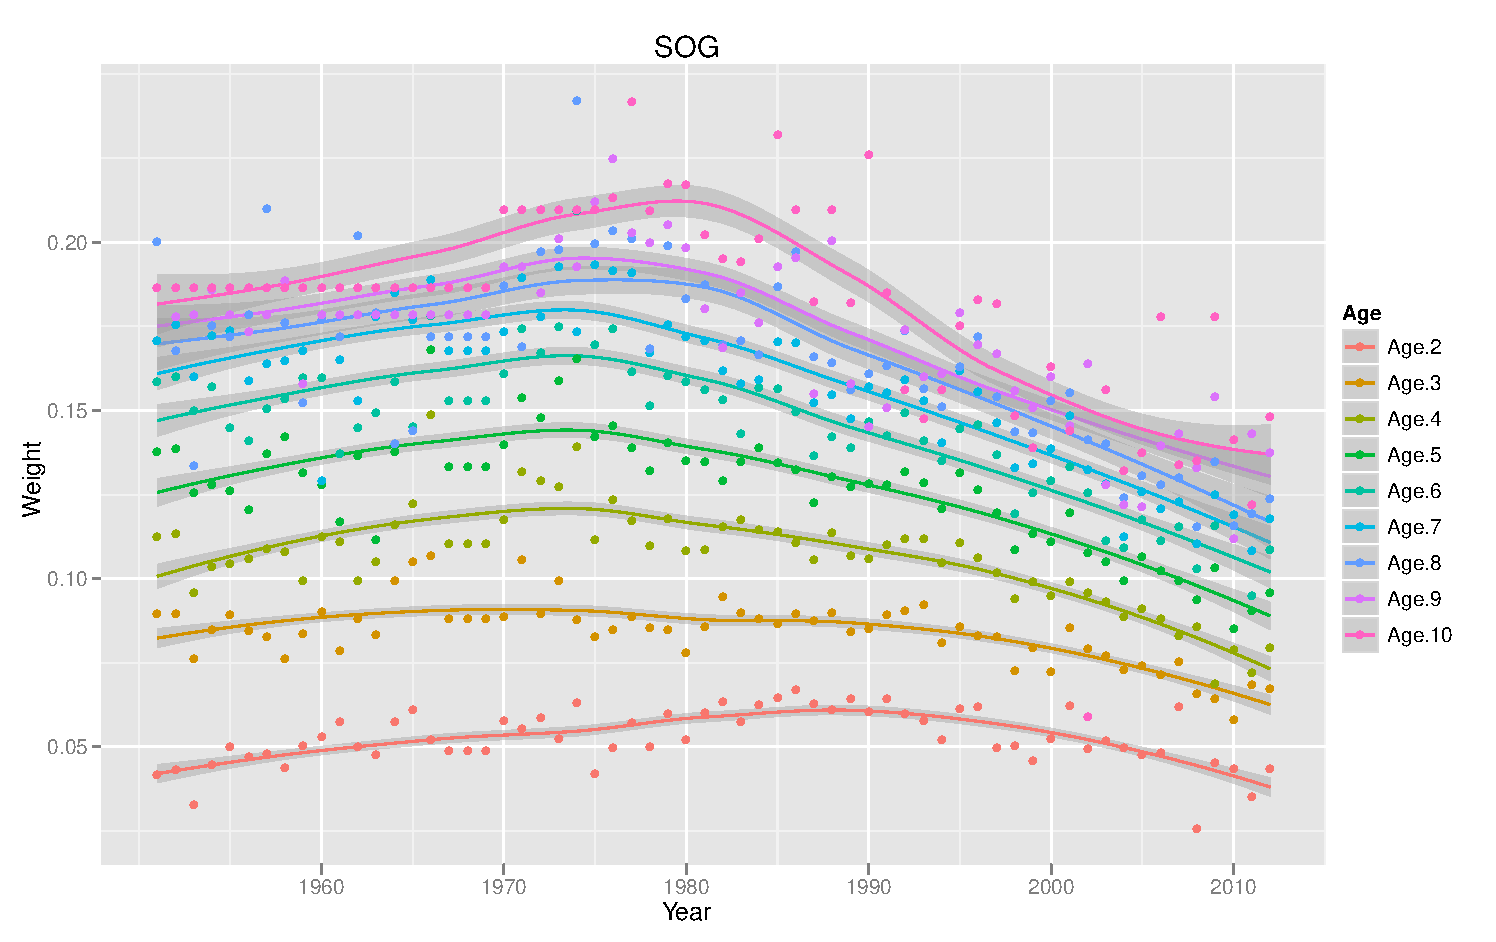
\includegraphics[scale=0.4]
		{../FIGS/iscam_fig_weight-at-age_SOG}
		\caption{Strait of Georgia: empirical weight-at-age (kg).}
	\end{figure}
	}
	%
	\only<5>{
	\begin{figure}[htbp]
		\centering
		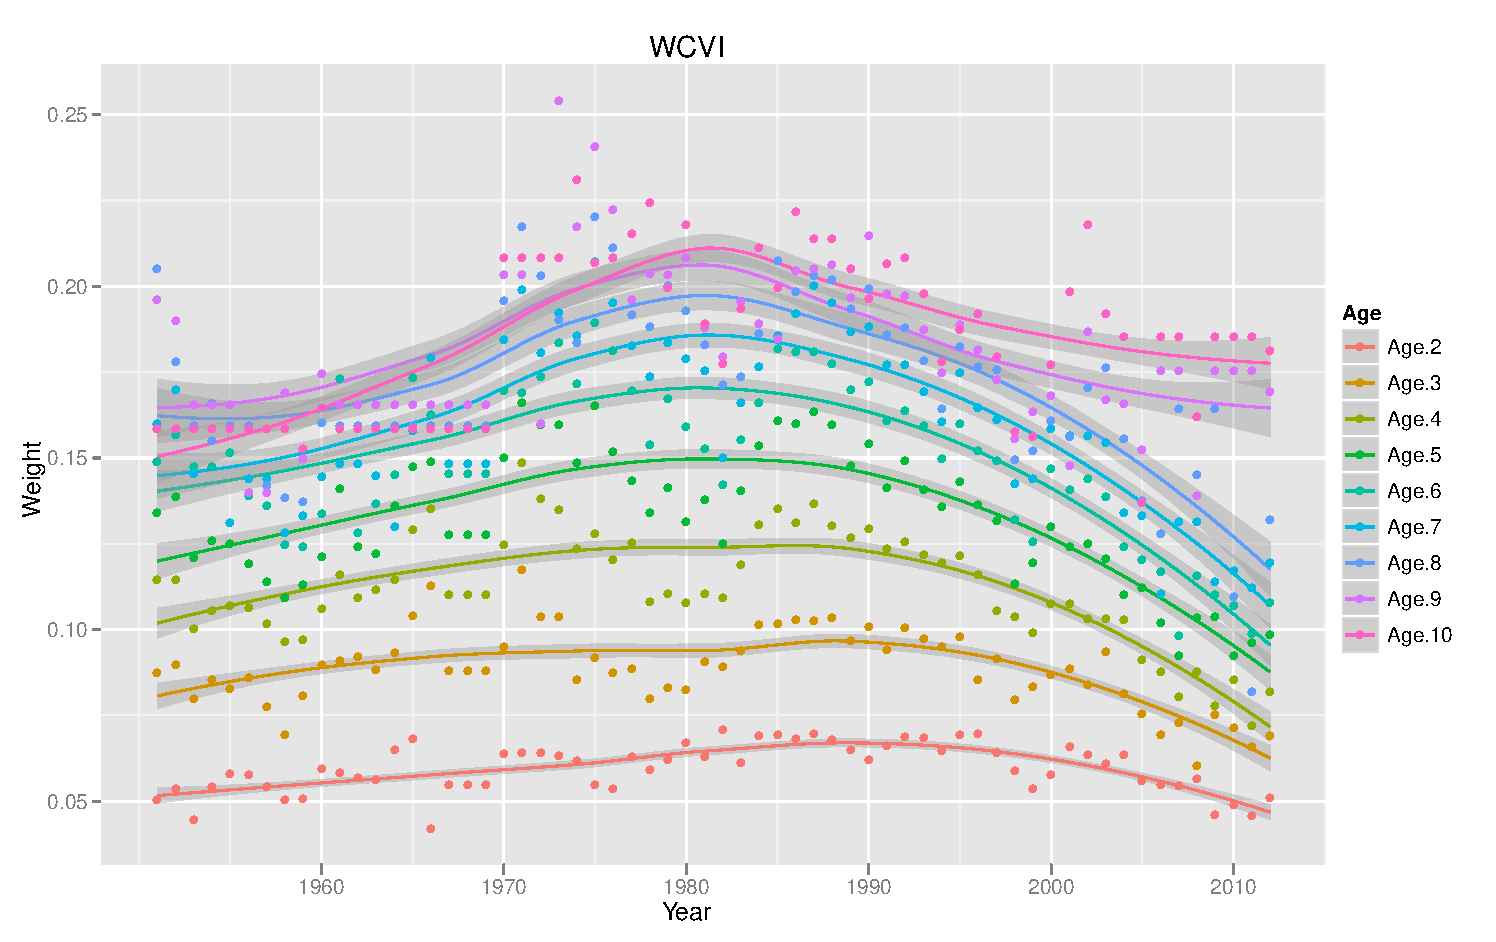
\includegraphics[scale=0.4]
		{../FIGS/iscam_fig_weight-at-age_WCVI}
		\caption{West Coast Vancouver Island: empirical weight-at-age (kg).}
	\end{figure}
	}
	%
\end{frame}
%
% subsection 2011_data (end)

\subsection{Analytical Methods} % (fold)
\label{sub:analytical_methods}
\begin{frame}[t]\frametitle{Analytics \& assumptions}
	\begin{itemize}
		\item<+-> All major and minor areas were assessed using  \iscam.
		\item<+-> Reported catch: CV = 0.005
		\item<+-> Spawn survey: proportional \& 100\% of $Z_t$.
		\item<+-> Dive survey more precise than surface survey.
		\item<+-> Fecundity $\propto$ mature weight-at-age.
		\item<+-> Seine gears: selectivity is asymptotic and time-invariant. 
		\item<+-|alert@+> Gillnet gear: logistic selectivity with weigth-at-age covariates.
		\item<+-|alert@+> $P(\ln(q_1),\ln(q_2)) \sim $ Normal($\mu=-0.569,\sigma=0.274$).
		\item<+-> Homogenous errors in age-composition (multivariate logistic).
		\item<+-> Age-samples $<$0.02 pooled in adjacent cohort.
	\end{itemize}
\end{frame}
% subsection analytical_methods (end)

% section part_ii (end)
